% UPDATES:
%DIF LATEXDIFF DIFFERENCE FILE
%DIF DEL old_2.tex              Fri Sep 22 18:24:40 2017
%DIF ADD vStrCueCoding_v1.tex   Fri Sep 22 17:59:29 2017
% Version 1.2 - JG initial import of text and figures from Google Drive, with edits

\documentclass[11pt]{article}

% packages
\usepackage{natbib}
\usepackage{graphicx}
\usepackage[nolists]{endfloat}
\usepackage{times}
\usepackage{ifthen}
\usepackage{parskip}
\usepackage[font=sf,labelfont=bf]{caption}
\usepackage{xspace}
\usepackage[pdftex]{color}
\usepackage{pdfcolmk}
\usepackage{fixltx2e} % for \textsubscript
%\usepackage{epstopdf}

% line numbers
\usepackage[left]{lineno}

% variable margins
\usepackage[left=2.5cm,top=2.5cm,bottom=3.5cm,right=2.5cm]{geometry}

% this helps figure placement
\renewcommand{\textfraction}{0.0}
\renewcommand{\topfraction}{1}
\renewcommand{\bottomfraction}{1}

% convert tif to png for pdf
%\epstopdfDeclareGraphicsRule{.tif}{png}{.png}{convert #1 \OutputFile}
%\AppendGraphicsExtensions{.tif}

% spacing
\setlength{\parindent}{0in} 
\setlength{\parskip}{2\baselineskip}
\linespread{2}
\renewcommand{\baselinestretch}{1.66}\normalsize

% definitions
\newcommand{\bsf}[1]{\textbf{#1}}
\newcommand{\sem}{S.E.M.\@\xspace}
\newcommand{\degree}{$^o$\@\xspace}
\makeatletter
\setlength{\@fptop}{0pt}
\makeatother

% bib
\bibliographystyle{apa}
\let\cite=\citep
\let\citeN=\citet
\let\citeNP=\citealt
\renewcommand{\bibfont}{\footnotesize}
\setlength{\bibsep}{2pt}
%DIF PREAMBLE EXTENSION ADDED BY LATEXDIFF
%DIF UNDERLINE PREAMBLE %DIF PREAMBLE
\RequirePackage[normalem]{ulem} %DIF PREAMBLE
\RequirePackage{color}\definecolor{RED}{rgb}{1,0,0}\definecolor{BLUE}{rgb}{0,0,1} %DIF PREAMBLE
\providecommand{\DIFadd}[1]{{\protect\color{blue}\uwave{#1}}} %DIF PREAMBLE
\providecommand{\DIFdel}[1]{{\protect\color{red}\sout{#1}}}                      %DIF PREAMBLE
%DIF SAFE PREAMBLE %DIF PREAMBLE
\providecommand{\DIFaddbegin}{} %DIF PREAMBLE
\providecommand{\DIFaddend}{} %DIF PREAMBLE
\providecommand{\DIFdelbegin}{} %DIF PREAMBLE
\providecommand{\DIFdelend}{} %DIF PREAMBLE
%DIF FLOATSAFE PREAMBLE %DIF PREAMBLE
\providecommand{\DIFaddFL}[1]{\DIFadd{#1}} %DIF PREAMBLE
\providecommand{\DIFdelFL}[1]{\DIFdel{#1}} %DIF PREAMBLE
\providecommand{\DIFaddbeginFL}{} %DIF PREAMBLE
\providecommand{\DIFaddendFL}{} %DIF PREAMBLE
\providecommand{\DIFdelbeginFL}{} %DIF PREAMBLE
\providecommand{\DIFdelendFL}{} %DIF PREAMBLE
\newcommand{\DIFscaledelfig}{0.5}
%DIF HIGHLIGHTGRAPHICS PREAMBLE %DIF PREAMBLE
\RequirePackage{settobox} %DIF PREAMBLE
\RequirePackage{letltxmacro} %DIF PREAMBLE
\newsavebox{\DIFdelgraphicsbox} %DIF PREAMBLE
\newlength{\DIFdelgraphicswidth} %DIF PREAMBLE
\newlength{\DIFdelgraphicsheight} %DIF PREAMBLE
% store original definition of \includegraphics %DIF PREAMBLE
\LetLtxMacro{\DIFOincludegraphics}{\includegraphics} %DIF PREAMBLE
\newcommand{\DIFaddincludegraphics}[2][]{{\color{blue}\fbox{\DIFOincludegraphics[#1]{#2}}}} %DIF PREAMBLE
\newcommand{\DIFdelincludegraphics}[2][]{% %DIF PREAMBLE
\sbox{\DIFdelgraphicsbox}{\DIFOincludegraphics[#1]{#2}}% %DIF PREAMBLE
\settoboxwidth{\DIFdelgraphicswidth}{\DIFdelgraphicsbox} %DIF PREAMBLE
\settoboxtotalheight{\DIFdelgraphicsheight}{\DIFdelgraphicsbox} %DIF PREAMBLE
\scalebox{\DIFscaledelfig}{% %DIF PREAMBLE
\parbox[b]{\DIFdelgraphicswidth}{\usebox{\DIFdelgraphicsbox}\\[-\baselineskip] \rule{\DIFdelgraphicswidth}{0em}}\llap{\resizebox{\DIFdelgraphicswidth}{\DIFdelgraphicsheight}{% %DIF PREAMBLE
\setlength{\unitlength}{\DIFdelgraphicswidth}% %DIF PREAMBLE
\begin{picture}(1,1)% %DIF PREAMBLE
\thicklines\linethickness{2pt} %DIF PREAMBLE
{\color[rgb]{1,0,0}\put(0,0){\framebox(1,1){}}}% %DIF PREAMBLE
{\color[rgb]{1,0,0}\put(0,0){\line( 1,1){1}}}% %DIF PREAMBLE
{\color[rgb]{1,0,0}\put(0,1){\line(1,-1){1}}}% %DIF PREAMBLE
\end{picture}% %DIF PREAMBLE
}\hspace*{3pt}}} %DIF PREAMBLE
} %DIF PREAMBLE
\LetLtxMacro{\DIFOaddbegin}{\DIFaddbegin} %DIF PREAMBLE
\LetLtxMacro{\DIFOaddend}{\DIFaddend} %DIF PREAMBLE
\LetLtxMacro{\DIFOdelbegin}{\DIFdelbegin} %DIF PREAMBLE
\LetLtxMacro{\DIFOdelend}{\DIFdelend} %DIF PREAMBLE
\DeclareRobustCommand{\DIFaddbegin}{\DIFOaddbegin \let\includegraphics\DIFaddincludegraphics} %DIF PREAMBLE
\DeclareRobustCommand{\DIFaddend}{\DIFOaddend \let\includegraphics\DIFOincludegraphics} %DIF PREAMBLE
\DeclareRobustCommand{\DIFdelbegin}{\DIFOdelbegin \let\includegraphics\DIFdelincludegraphics} %DIF PREAMBLE
\DeclareRobustCommand{\DIFdelend}{\DIFOaddend \let\includegraphics\DIFOincludegraphics} %DIF PREAMBLE
\LetLtxMacro{\DIFOaddbeginFL}{\DIFaddbeginFL} %DIF PREAMBLE
\LetLtxMacro{\DIFOaddendFL}{\DIFaddendFL} %DIF PREAMBLE
\LetLtxMacro{\DIFOdelbeginFL}{\DIFdelbeginFL} %DIF PREAMBLE
\LetLtxMacro{\DIFOdelendFL}{\DIFdelendFL} %DIF PREAMBLE
\DeclareRobustCommand{\DIFaddbeginFL}{\DIFOaddbeginFL \let\includegraphics\DIFaddincludegraphics} %DIF PREAMBLE
\DeclareRobustCommand{\DIFaddendFL}{\DIFOaddendFL \let\includegraphics\DIFOincludegraphics} %DIF PREAMBLE
\DeclareRobustCommand{\DIFdelbeginFL}{\DIFOdelbeginFL \let\includegraphics\DIFdelincludegraphics} %DIF PREAMBLE
\DeclareRobustCommand{\DIFdelendFL}{\DIFOaddendFL \let\includegraphics\DIFOincludegraphics} %DIF PREAMBLE
%DIF END PREAMBLE EXTENSION ADDED BY LATEXDIFF

\begin{document}

{\Large\bf Coding of behaviorally relevant and irrelevant cue features in the nucleus accumbens}

{\bf Authors}: Jimmie M.\ Gmaz\textsuperscript{1}, James
E.\ Carmichael\textsuperscript{1}, Matthijs A.\ A.\ van der
Meer\textsuperscript{1*}

\textsuperscript{1}Department of Psychological and Brain Sciences,
Dartmouth College, Hanover NH
03755\\ 

\textsuperscript{*}Correspondence should be addressed to MvdM,
Department of Psychological and Brain Sciences, Dartmouth College, 3
Maynard St, Hanover, NH 03755. E-mail: {\sffamily mvdm@dartmouth.edu}.

\textbf{Number of Figures:} 11\\
\textbf{Number of Tables:} 1\\
\textbf{Total Word Count:} ?\\
\textbf{Abstract Word Count:} ?\\
\textbf{Introduction Word Count:} ?\\
\textbf{Discussion Word Count:} ?\\

\textbf{Acknowledgments}: We thank Nancy Gibson, Martin Ryan and Jean
Flanagan for animal care, and Min-Ching Kuo and
Alyssa Carey for technical assistance. This work was supported by
Dartmouth College (Dartmouth Fellowship to JMG and JEC, and start-up funds to
MvdM) and the Natural Sciences and Engineering Research Council
(NSERC) of Canada (Discovery Grant award to MvdM, Canada Graduate
Scholarship to JMG).

\textbf{Conflict of Interest}: The authors declare no competing
financial interests.\\

\newpage
\linenumbers

\section*{Abstract}

to do

\section*{Significance Statement (120 words)}

to do

\newpage

\section*{Introduction}
% Version 1.2 - imported from Google Drive
% To do JG: refine (e.g. make more explicit the tie to the schematic), add references

Theories of nucleus accumbens (NAc) function generally agree that this brain structure contributes to motivated behavior, with some emphasizing a role in learning from reward prediction errors (Joel, Doya, Schultz; see also the addiction literature on the effects of drug rewards; Nestler, Kalivas; Carelli) and others a role in the modulation of ongoing behavior through stimuli associated with motivationally relevant outcomes (invigorating, directing; Nicola, Floresco, Salamone). These proposals echo similar ideas on the functions of the neuromodulator dopamine (Schultz, Berridge, Maia/Frank, Cools), with which the NAc is tightly linked functionally as well as anatomically (Haber, Sesack, Takahashi).

Much of our understanding of NAc function comes from studies of how cues that predict motivationally relevant outcomes (e.g. reward) influence behavior and neural activity in the NAc. Task designs that associate such cues with rewarding outcomes provide a convenient access point eliciting conditioned responses such as sign-tracking and goal-tracking (Robinson), pavlovian-instrumental transfer (Balleine) and enhanced response vigor (Niv; McGinty), which tend to be affected by NAc manipulations (Flagel, Balleine, Chang; although not always straightforwardly: Hauber, Chang). Similarly, analysis of reward prediction errors typically proceeds by establishing an association between a cue and subsequent reward, with NAc responses transferring from outcome to the cue with learning (Schultz, Schoenbaum, Carelli). WHAT ABOUT HUMAN WORK

Surprisingly, although substantial work has been done on the coding of outcomes predicted by such cues (e.g. reward value; Hollerman/Schultz, Roesch, Day; reward identity; Cooch), much less is known about how reward-predictive cues themselves are encoded in the NAc (Hayden from primate realm). This is an important issue for at least two reasons. First, in reinforcement learning, motivationally relevant outcomes are typically temporally delayed relative to the cues that predict them. In order to solve the problem of assigning credit (or blame) across such temporal gaps, some trace of preceding activity needs to be maintained (Maia?). Since NAc is a primary target of DA signals interpretable as RPEs, and NAc lesions impair RPEs related to timing, its activity trace will help determine what can be learned when RPEs arrive (Takahashi).

Second, for ongoing behavior, the relevance of cues typically depends on “context”. In experimental settings, context may include the identity of a preceding cue (occasion setter, Holland, Kesner), spatial or configural arrangements (Good/Honey, Eichenbaum), and unsignaled rules as occurs in set shifting and other cognitive control tasks (CITE). In such situations, the question arises how selective, context-dependent processing of reward-predictive cues is implemented. For instance, is there a “gate” prior to NAc, or are all cues represented in NAc but their current values dynamically updated (FitzGerald; WHAT ARE SOME THEORETICAL POSITIONS ON THIS)? 

Thus, both from a learning and a flexible performance perspective, it is of interest to determine how cue identity is represented in the brain, with NAc of particular interest given its anatomical and functional position at the center of motivational systems. We sought to determine whether cue features signalling identity are represented in the NAc, and if cue identity is represented alongside other motivationally relevant variables, such as cue value (Figure \ref{fig:schematic}). To address this question, we designed an experiment in which multiple, distinct sets of cues predicted the same outcome. We recorded the activity of NAc neurons as rats performed this task. 

\begin{figure}
[h]
\centering
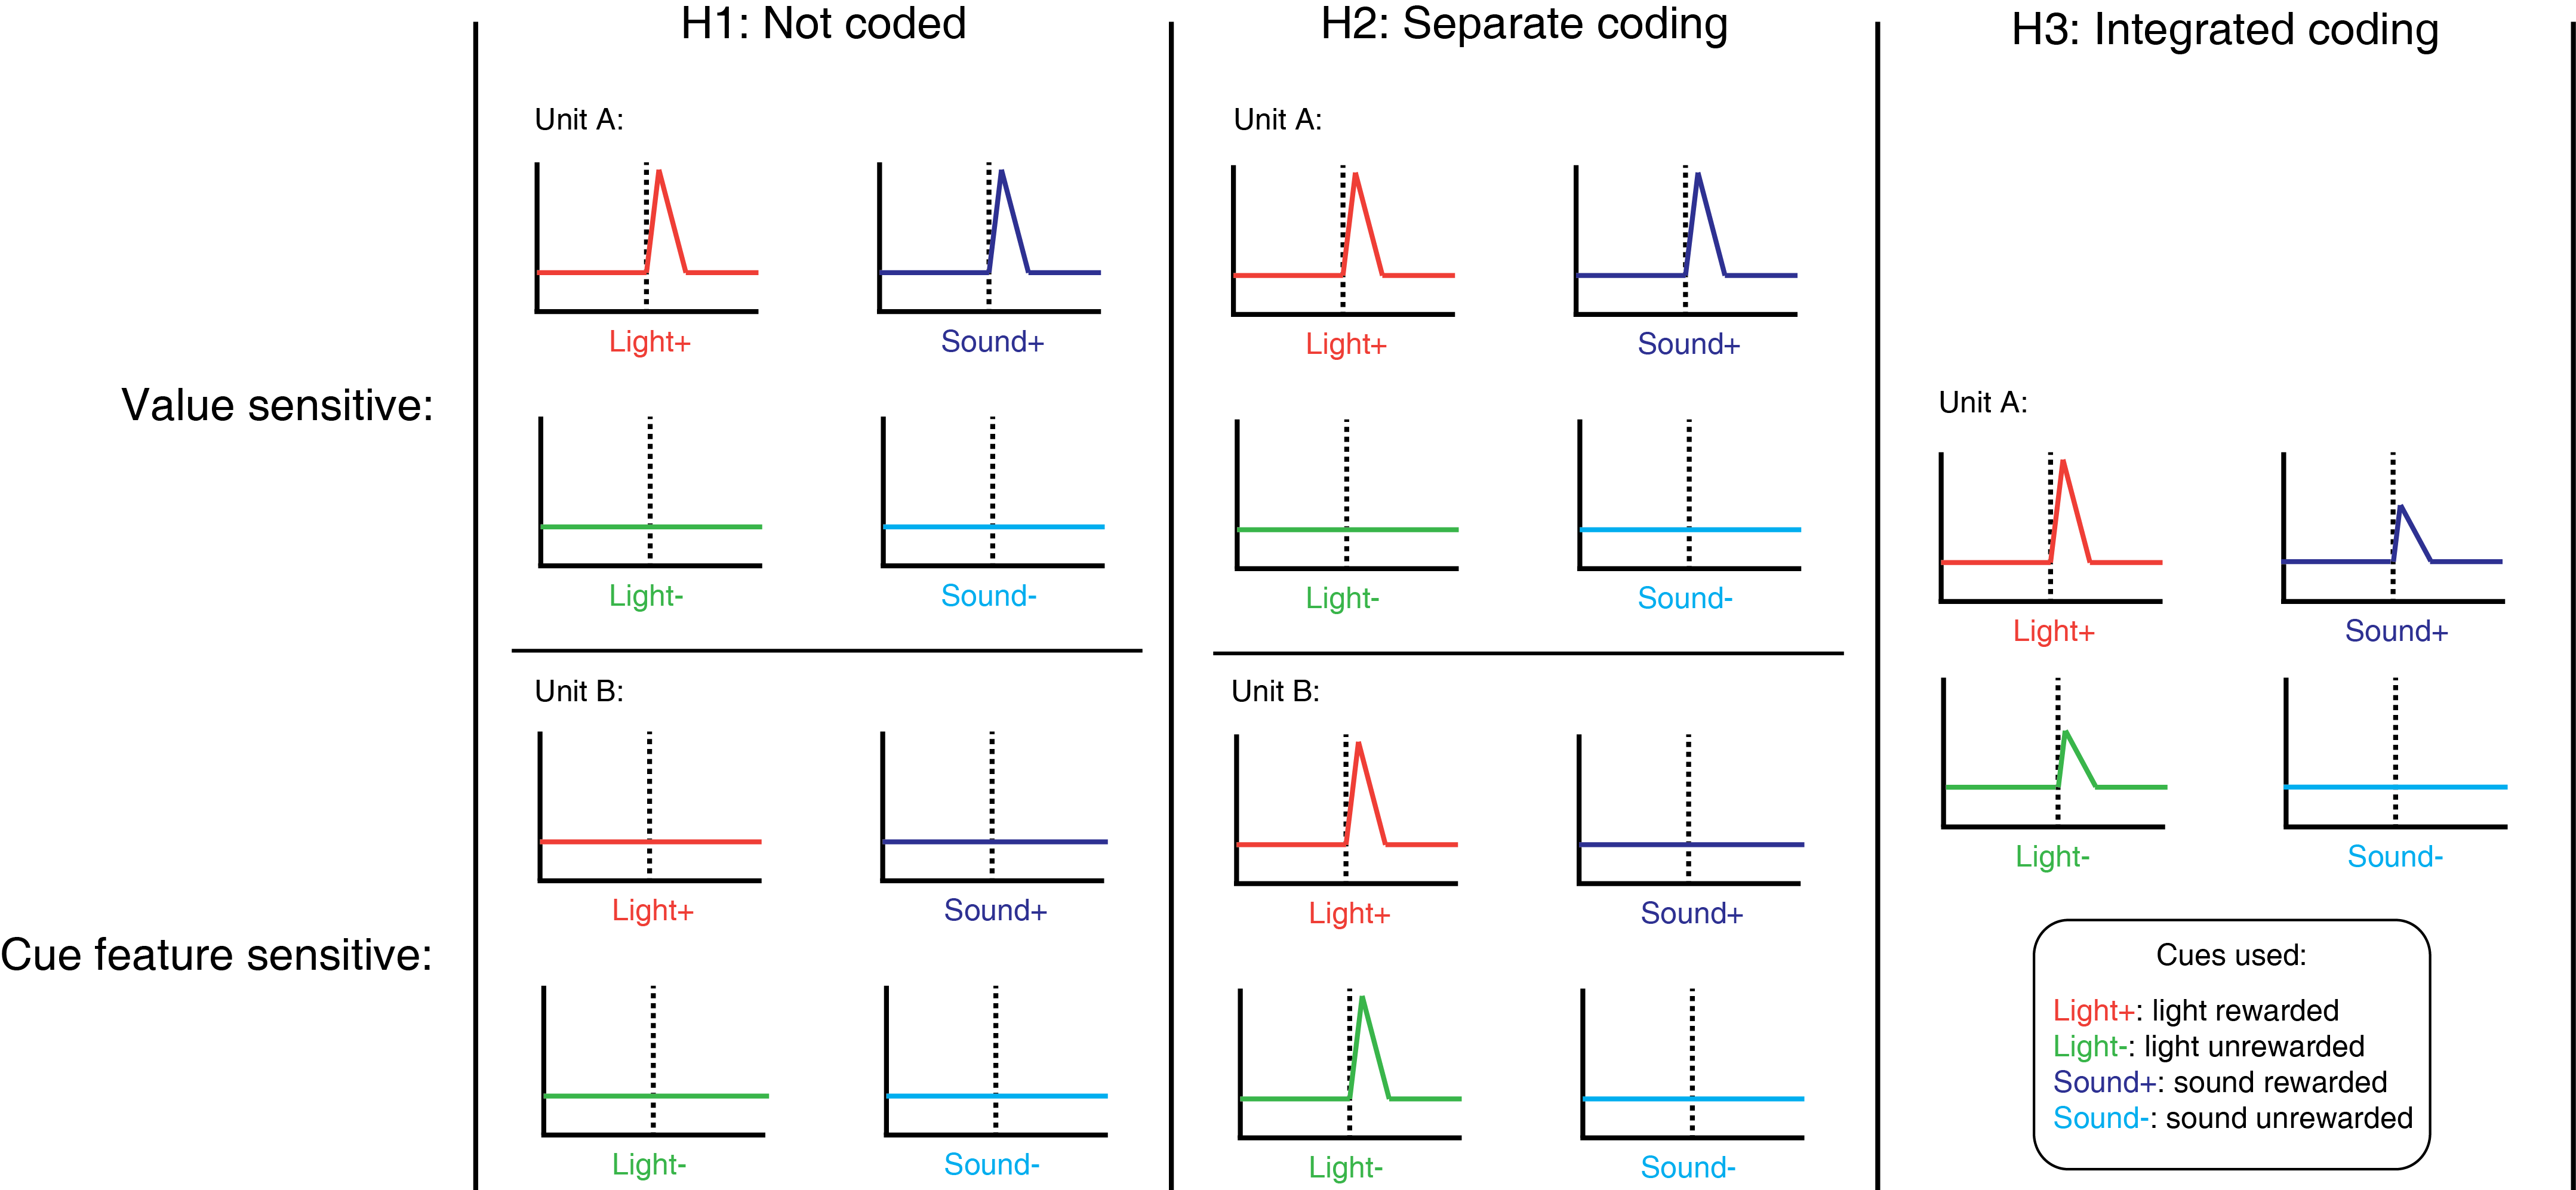
\includegraphics[width=\textwidth]{Fig 1 - Schematic neural.png}
\caption{\DIFdelbeginFL \DIFdelFL{Neural schematic}\DIFdelendFL \DIFaddbeginFL \DIFaddFL{Schematic of potential coding strategies employed by single units in the NAc. Coding of identifying cue features could occur either be absent in the NAc (left), occur independently of encoding of motivationally relevant variables like expected value or subsequent vigor (middle), and/or be integrated with coding of other motivationally relevant variables (right).}\DIFaddendFL }
\label{fig:schematic}

\end{figure}
\section*{Methods}
%DIF < Version 1.2 - imported from Google Drive
%DIF < To do JG: add stats for pop level and tiling stats
%DIF > Version 1.3 - post Matt round 1 edits
%DIF > To do JG: add stats for pop level and tiling

{\bf Subjects:}

Adult male Long-Evans rats (n = 4, Charles River, Saint Constant, QC) were used as subjects. Rats were individually housed with a 12/12-h light-dark cycle, and tested during the light cycle. Rats were food deprived to 85-90\% of their free feeding weight (weight at time of implantation was 440 - 470 g), and water restricted 4-6 hours before testing. All experimental procedures were approved by the the University of Waterloo Animal Care Committee (protocol\# 11-06) and carried out in accordance with Canadian Council for Animal Care (CCAC) guidelines. 

{\bf Overall timeline:}

Each subject was first handled for seven days where they were exposed to the running room, the sucrose solution, and the click of the valves upon approach to the receptacles. They were then shaped to run on the task for seven days where they were restricted to running in the clockwise direction by presenting a physical barrier to running counterclockwise. Rats underwent hyperdrive implantation after showing discrimination of approach behavior for rewarded and unrewarded cues for three consecutive days according to a chi square test. Rats were allowed to recover for a minimum of five days before being retrained on the task, and recording began once performance returned to pre-surgery levels. Upon completion of recording, animals were sacrificed and recording sites were histologically confirmed.

{\bf Behavioral task and training:} 

Rats were trained to run clockwise on an elevated, square-shaped track (100x100 cm) containing four possible reward locations (Figure \ref{fig:task}). Rats initiated a trial by running down the length of an arm, and triggering a photobeam located 24 cm from the start of each arm. Upon trial initiation, a \DIFaddbegin \DIFadd{light or sound }\DIFaddend cue was presented that signaled the presence of absence of a 12\% sucrose water reward (0.1 mL) at the upcoming site. A trial was classified as an approach trial if the rat turned left at the decision point and made a nosepoke at the reward receptacle (40 cm from the decision point), while trials were classified as a skip trial if the rat instead turned right at the decision point and triggered the photobeam to initiate the following trial. There was a 1 second delay \DIFdelbegin \DIFdel{from }\DIFdelend \DIFaddbegin \DIFadd{between }\DIFaddend a rewarded nosepoke and \DIFaddbegin \DIFadd{subsequent }\DIFaddend reward delivery. \DIFaddbegin \DIFadd{Trial length was determined by measuring the length of time from cue onset until nosepoke or the start of the following trial. Trials could only be initiated through clockwise progression through the series of arms, and each entry into the subsequent arm on the track counted as a trial. }\DIFaddend Each day rats were trained in both a light and sound block for 100 trials each. Within a block, one cue signaled reward was available on that trial, while the other signaled reward was not available. Light block cues were a flashing white light, and a constant yellow light. Sound block cues were a 2 kHz sine wave and a 8 kHz sine wave whose amplitude was modulated from 0 to maximum by a 2 Hz sine wave. Reward-cue associations were counterbalanced across rats. Cue presentation was pseudorandomized so that the same cue could not be presented more than twice in a row. Block order within each day was also pseudorandomized, such that the rat could \DIFdelbegin \DIFdel{not start with the block within a session }\DIFdelend \DIFaddbegin \DIFadd{begin a session with the same block for }\DIFaddend more than two days in a row. Each training or testing day consisted of a 5 minute pre-session period on a pedestal, followed by the first block, then the second block, then a 5 minute post-session period on the pedestal. Accuracy was determined by the proportion of trials a rat approached each cue. Perfect performance would be 100\% approach on “approach” trials (reward available), and 0\% approach on “skip” trials (no reward available). \DIFdelbegin \DIFdel{Trial length was determined by measuring the length of time from cue onset until nosepoke or the start of the following trial. }\DIFdelend Rats were trained daily until they could distinguish between the rewarded and unrewarded cues for both light and sound blocks for three consecutive days according to a chi-square test, at which point they underwent surgery. Furthermore, we generated linear mixed effects models to \DIFdelbegin \DIFdel{look at }\DIFdelend \DIFaddbegin \DIFadd{investigate }\DIFaddend the relationships between cue type and our behavioral variables\DIFdelbegin \DIFdel{. Cue }\DIFdelend \DIFaddbegin \DIFadd{, with cue }\DIFaddend type was used as a fixed effect, and \DIFdelbegin \DIFdel{we had }\DIFdelend \DIFaddbegin \DIFadd{the addtion of }\DIFaddend an intercept for rat identity as a random effect. Average proportion of trials approached and trial length for a session were used as response variables. Contribution of cue type to behavior was determined by comparing the full model to a model with cue type removed for each behavioral variable. 

\begin{figure}[h]
\centering
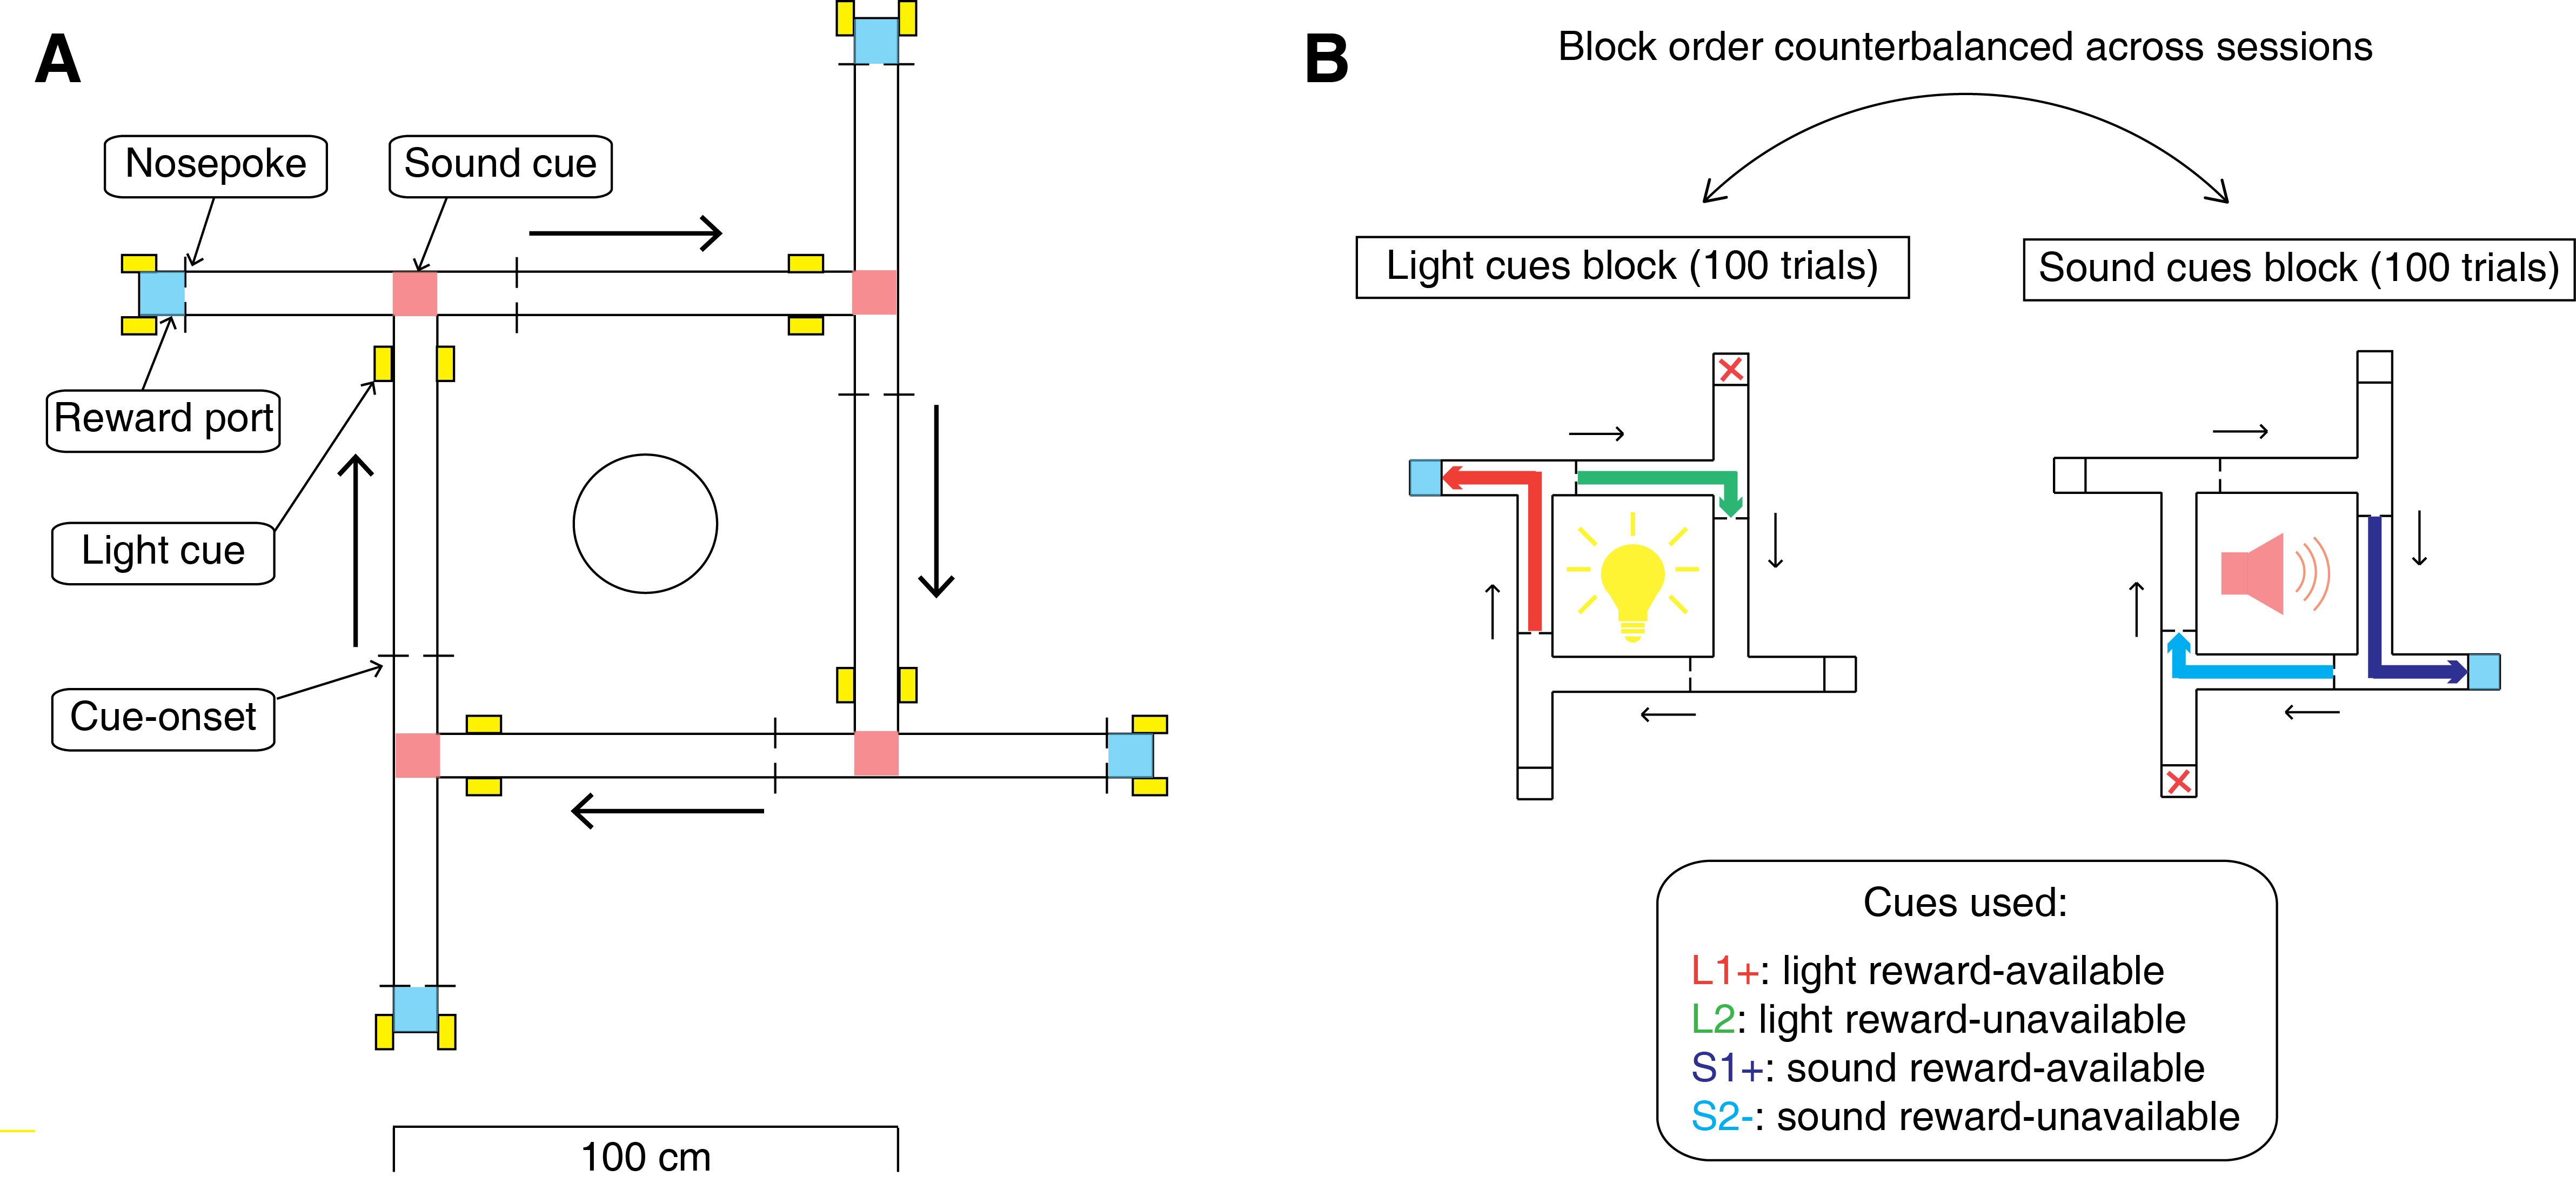
\includegraphics[width=\textwidth]{Fig 2 - Schematic task.png}
\caption{\DIFdelbeginFL \DIFdelFL{Task schematic}\DIFdelendFL \DIFaddbeginFL \DIFaddFL{Schematic of behavioral task and procedure used in current study. A session was started with a 5 minute recording period on a pedestal place in the center of the apparatus (left). Rats then underwent two blocks of a cue discrimination task on a square track where they had to dissociate between a rewarded and unrewarded cue for a set of light cues and a set of sound cues for a target of 100 trials each (middle). Rats ran clockwise on the square track, and upon presentation of the cue had to turn left at the choice point to receive reward for a rewarded cue (approach trial; red and navy blue in figure), or turn right at the choice point to initiate the following trial for an unrewarded cue (skip trial; green and cyan in figure). Ordering of the light and sound blocks was counterbalanced across sessions. A session ended with another 5 minute recording period on the pedestal (right).}\DIFaddendFL }
\label{fig:task}
\end{figure}
{\bf Surgery:}

Surgical procedures were as described previously (Malhotra et al., 2015). Briefly, animals were anesthetized with isoflurane, induced with 5\% in medical grade oxygen and maintained at 2\% throughout the surgery (~0.8 L/min). Rats were then chronically implanted with a “hyperdrive” consisting of 16 independently drivable tetrodes, either all 16 targeted for the right NAc (AP +1.4 mm and ML +1.6 mm, relative to bregma; Paxinos and Watson, 2005), or 12 in the right NAc and 4 targeted at the mPFC (AP +3.0 mm and ML +0.6 mm, relative to bregma; only data from NAc tetrodes were analyzed). Following surgery, all animals were given a least five days to recover and lower tetrodes to the target (DV -6.0 mm) before being reintroduced to the behavioral task.

{\bf Data acquisition and preprocessing:}

After recovery, rats were placed back on the task for recording. NAc signals were acquired at 20 kHz with a RHA2132 v0810 preamplifier (Intan) and a KJE-1001/KJD-1000 data acquisition system (Amplipex). Signals were referenced against a tetrode placed in the corpus callosum above the NAc.

Candidate spikes for sorting into putative single units were obtained by band-pass filtering the data between 600-9000 Hz, thresholding and aligning the peaks (UltraMegaSort2k, Hull et al., 2011). Spike waveforms were then clustered with KlustaKwik using energy and the first derivative of energy as features\DIFdelbegin \DIFdel{(peak, valley, peak index, wave PC1, time were used as extra features, does this need to be included?), }\DIFdelend \DIFaddbegin \DIFadd{, }\DIFaddend and manually sorted into units (MClust 3.5, A.D. Redish et al.). Isolated units containing a minimum of 200 spikes within a session were included for subsequent analysis. Units were classified as high firing neurons if they had high tonic firing rates marked by an absence of interspike intervals (ISIs) $>$ 2 s, while medium spiny neurons had a combination of ISIs $>$ 2 s and phasic activity with shorter ISIs (Barnes 2005, Atallah 2014). 

{\bf Data analysis:}

\DIFdelbegin \DIFdel{Average firing rates }\DIFdelend \DIFaddbegin \DIFadd{To investigate the contribution of various cue features on NAc firing rates we first determined whether firing rates for a unit were modulated by the onset of a cue by collapsing across all cues and comparing the firing rates }\DIFaddend for \DIFdelbegin \DIFdel{a session were generated for }\DIFdelend the 1 s preceding cue-onset \DIFdelbegin \DIFdel{, and }\DIFdelend \DIFaddbegin \DIFadd{with }\DIFaddend the 1 s following cue-onset. Single units were considered to be cue-responsive if \DIFdelbegin \DIFdel{both }\DIFdelend \DIFaddbegin \DIFadd{a Wilcoxon signed-rank test comparing pre- and post-cue firing had a p $<$ .01. (Excluded: ‘}\DIFaddend the mean firing rate difference between pre- and post-cue onset was within the lower or upper 2.5\% of a shuffled distribution\DIFdelbegin \DIFdel{, and a Wilcoxon signed-rank test comparing pre- and post-cue firing was p $<$ .01. Units where a Mann-Whitney U test revealed a drift in firing rate between the first and second half of the trails in either task block were excluded from analysis}\DIFdelend \DIFaddbegin \DIFadd{’, as there is redundancy using both, and I did both because I was paranoid about just using one. )}\DIFaddend . Cue-modulated \DIFdelbegin \DIFdel{responses were }\DIFdelend \DIFaddbegin \DIFadd{units were then }\DIFaddend classified as either increasing or decreasing \DIFaddbegin \DIFadd{in response to the cue }\DIFaddend if the post-cue activity was higher or lower than the pre-cue activity, respectively. 
\DIFdelbegin \DIFdel{A }\DIFdelend \DIFaddbegin 

\DIFadd{To determine the relative contribution of various task parameters to firing rate variance for units whose firing was modulated by cue-onset (as in Figures \ref{fig:examples},\ref{fig:GLM}), a forward selection }\DIFaddend stepwise general linear model (GLM) was \DIFdelbegin \DIFdel{then fit to }\DIFdelend \DIFaddbegin \DIFadd{fit to each }\DIFaddend cue-responsive \DIFdelbegin \DIFdel{units using cue }\DIFdelend \DIFaddbegin \DIFadd{unit. Cue }\DIFaddend modality, cue location, cue outcome, approach behavior, trial length, trial number, and trial history \DIFaddbegin \DIFadd{were used }\DIFaddend as predictors, and \DIFaddbegin \DIFadd{the }\DIFaddend 1 s post-cue firing rate as the response variable. Units were classified as being modulated by a given task parameter if addition of the parameter significantly \DIFdelbegin \DIFdel{improvement }\DIFdelend \DIFaddbegin \DIFadd{improved }\DIFaddend model fit using deviance as the criterion (p $<$ .01). A comparison of the R-squared value between the \DIFdelbegin \DIFdel{complete }\DIFdelend \DIFaddbegin \DIFadd{final }\DIFaddend model and the \DIFaddbegin \DIFadd{final }\DIFaddend model minus the predictor of interest was used to determine the amount of firing rate variance explained by the addition of that predictor \DIFdelbegin \DIFdel{. Spike }\DIFdelend \DIFaddbegin \DIFadd{for a given unit. 
}

\DIFadd{To better visualize responses to cues and enable subsequent population level analyses (as in Figures \ref{fig:examples},\ref{fig:pop},\ref{fig:tiling}), spike }\DIFaddend trains were convolved with a Gaussian kernel\DIFdelbegin \DIFdel{(Matt: do I need to show or say something that convolving the spike trains did not interfere too much with the response around stimulus onset?)}\DIFdelend , and peri-event time histograms (PETHs) were generated by taking the average of the convolved spike trains across trials for a given task condition. \DIFdelbegin \DIFdel{To analyze }\DIFdelend \DIFaddbegin \DIFadd{For analysis of }\DIFaddend population-level responses for cue features \DIFaddbegin \DIFadd{(Figure \ref{fig:pop})}\DIFaddend , convolved spike trains for all \DIFdelbegin \DIFdel{cells where a specified cue feature }\DIFdelend \DIFaddbegin \DIFadd{units where cue modality, cue location, or cue outcome }\DIFaddend explained a significant portion of firing rate variance were z-scored. \DIFdelbegin \DIFdel{Normalized }\DIFdelend \DIFaddbegin \DIFadd{Within a given cue feature, normalized }\DIFaddend spike trains were \DIFaddbegin \DIFadd{then }\DIFaddend separated according to \DIFaddbegin \DIFadd{the }\DIFaddend preferred and non-preferred cue condition \DIFaddbegin \DIFadd{(e.g. light vs sound block)}\DIFaddend , and averaged across \DIFdelbegin \DIFdel{cells }\DIFdelend \DIFaddbegin \DIFadd{units }\DIFaddend to generate population-level averages.
\DIFdelbegin \DIFdel{STATISTICAL TEST? }\DIFdelend \DIFaddbegin 

\DIFaddend To visualize NAc representation of task space within cue conditions, normalized spike trains for all \DIFdelbegin \DIFdel{cells }\DIFdelend \DIFaddbegin \DIFadd{units }\DIFaddend were ordered by the location of their maximum or minimum firing rate for a specified cue condition \DIFaddbegin \DIFadd{(Figure \ref{fig:tiling})}\DIFaddend . To compare representation of task space across cue conditions \DIFaddbegin \DIFadd{for a cue feature}\DIFaddend , the ordering of \DIFdelbegin \DIFdel{cells taken from one condition }\DIFdelend \DIFaddbegin \DIFadd{units derived for one condition (e.g. light block) }\DIFaddend was then applied to the normalized spike trains \DIFdelbegin \DIFdel{from the condition to be compared.STATISTICAL TEST? The same cells identified as being responsive to cue-onset were also analyzed }\DIFdelend \DIFaddbegin \DIFadd{for the other condition (e.g. sound block). 
}

\DIFadd{To identify the responsivity of units to different cue features }\DIFaddend at the time of \DIFaddbegin \DIFadd{a }\DIFaddend nosepoke into a reward receptacle\DIFdelbegin \DIFdel{using similar methods.
}\DIFdelend \DIFaddbegin \DIFadd{, the same cue-responsive units from the cue-onset analyses were analyzed at the time of nosepoke using identical analysis techniques (Figures \ref{fig:NP_GLM},\ref{fig:NP_pop},\ref{fig:NP_tiling}).
}

\DIFadd{Given that some of our analyses compare firing rates across time, particularly comparisons across blocks, we sought to exclude units with unstable firing rates that would generate spurious results reflecting a drift in firing rate over time unrelated to our task. To do this we ran a Mann-Whitney U test comparing the cue-evoked firing rates for the first and second half of trials within a block, and excluded units from analysis that showed a significant change for either block.  }\DIFaddend All analyses were completed in MATLAB R2015a, and the code is available on GitHub.


{\bf Histology:}

Upon completion of the experiment, rats were anesthetized with 5\% isoflurane, then asphyxiated with carbon dioxide. Transcardial perfusions were performed, and brains were fixed and removed. Brains were sliced in 50 um coronal sections and stained with thionin. Slices were visualized under light microscopy, \DIFdelbegin \DIFdel{and }\DIFdelend tetrode placement was determined\DIFaddbegin \DIFadd{, and electrodes with recording locations in the NAc were analyzed }\DIFaddend (Figure \ref{fig:histo}).

\begin{figure}
[h]
\centering
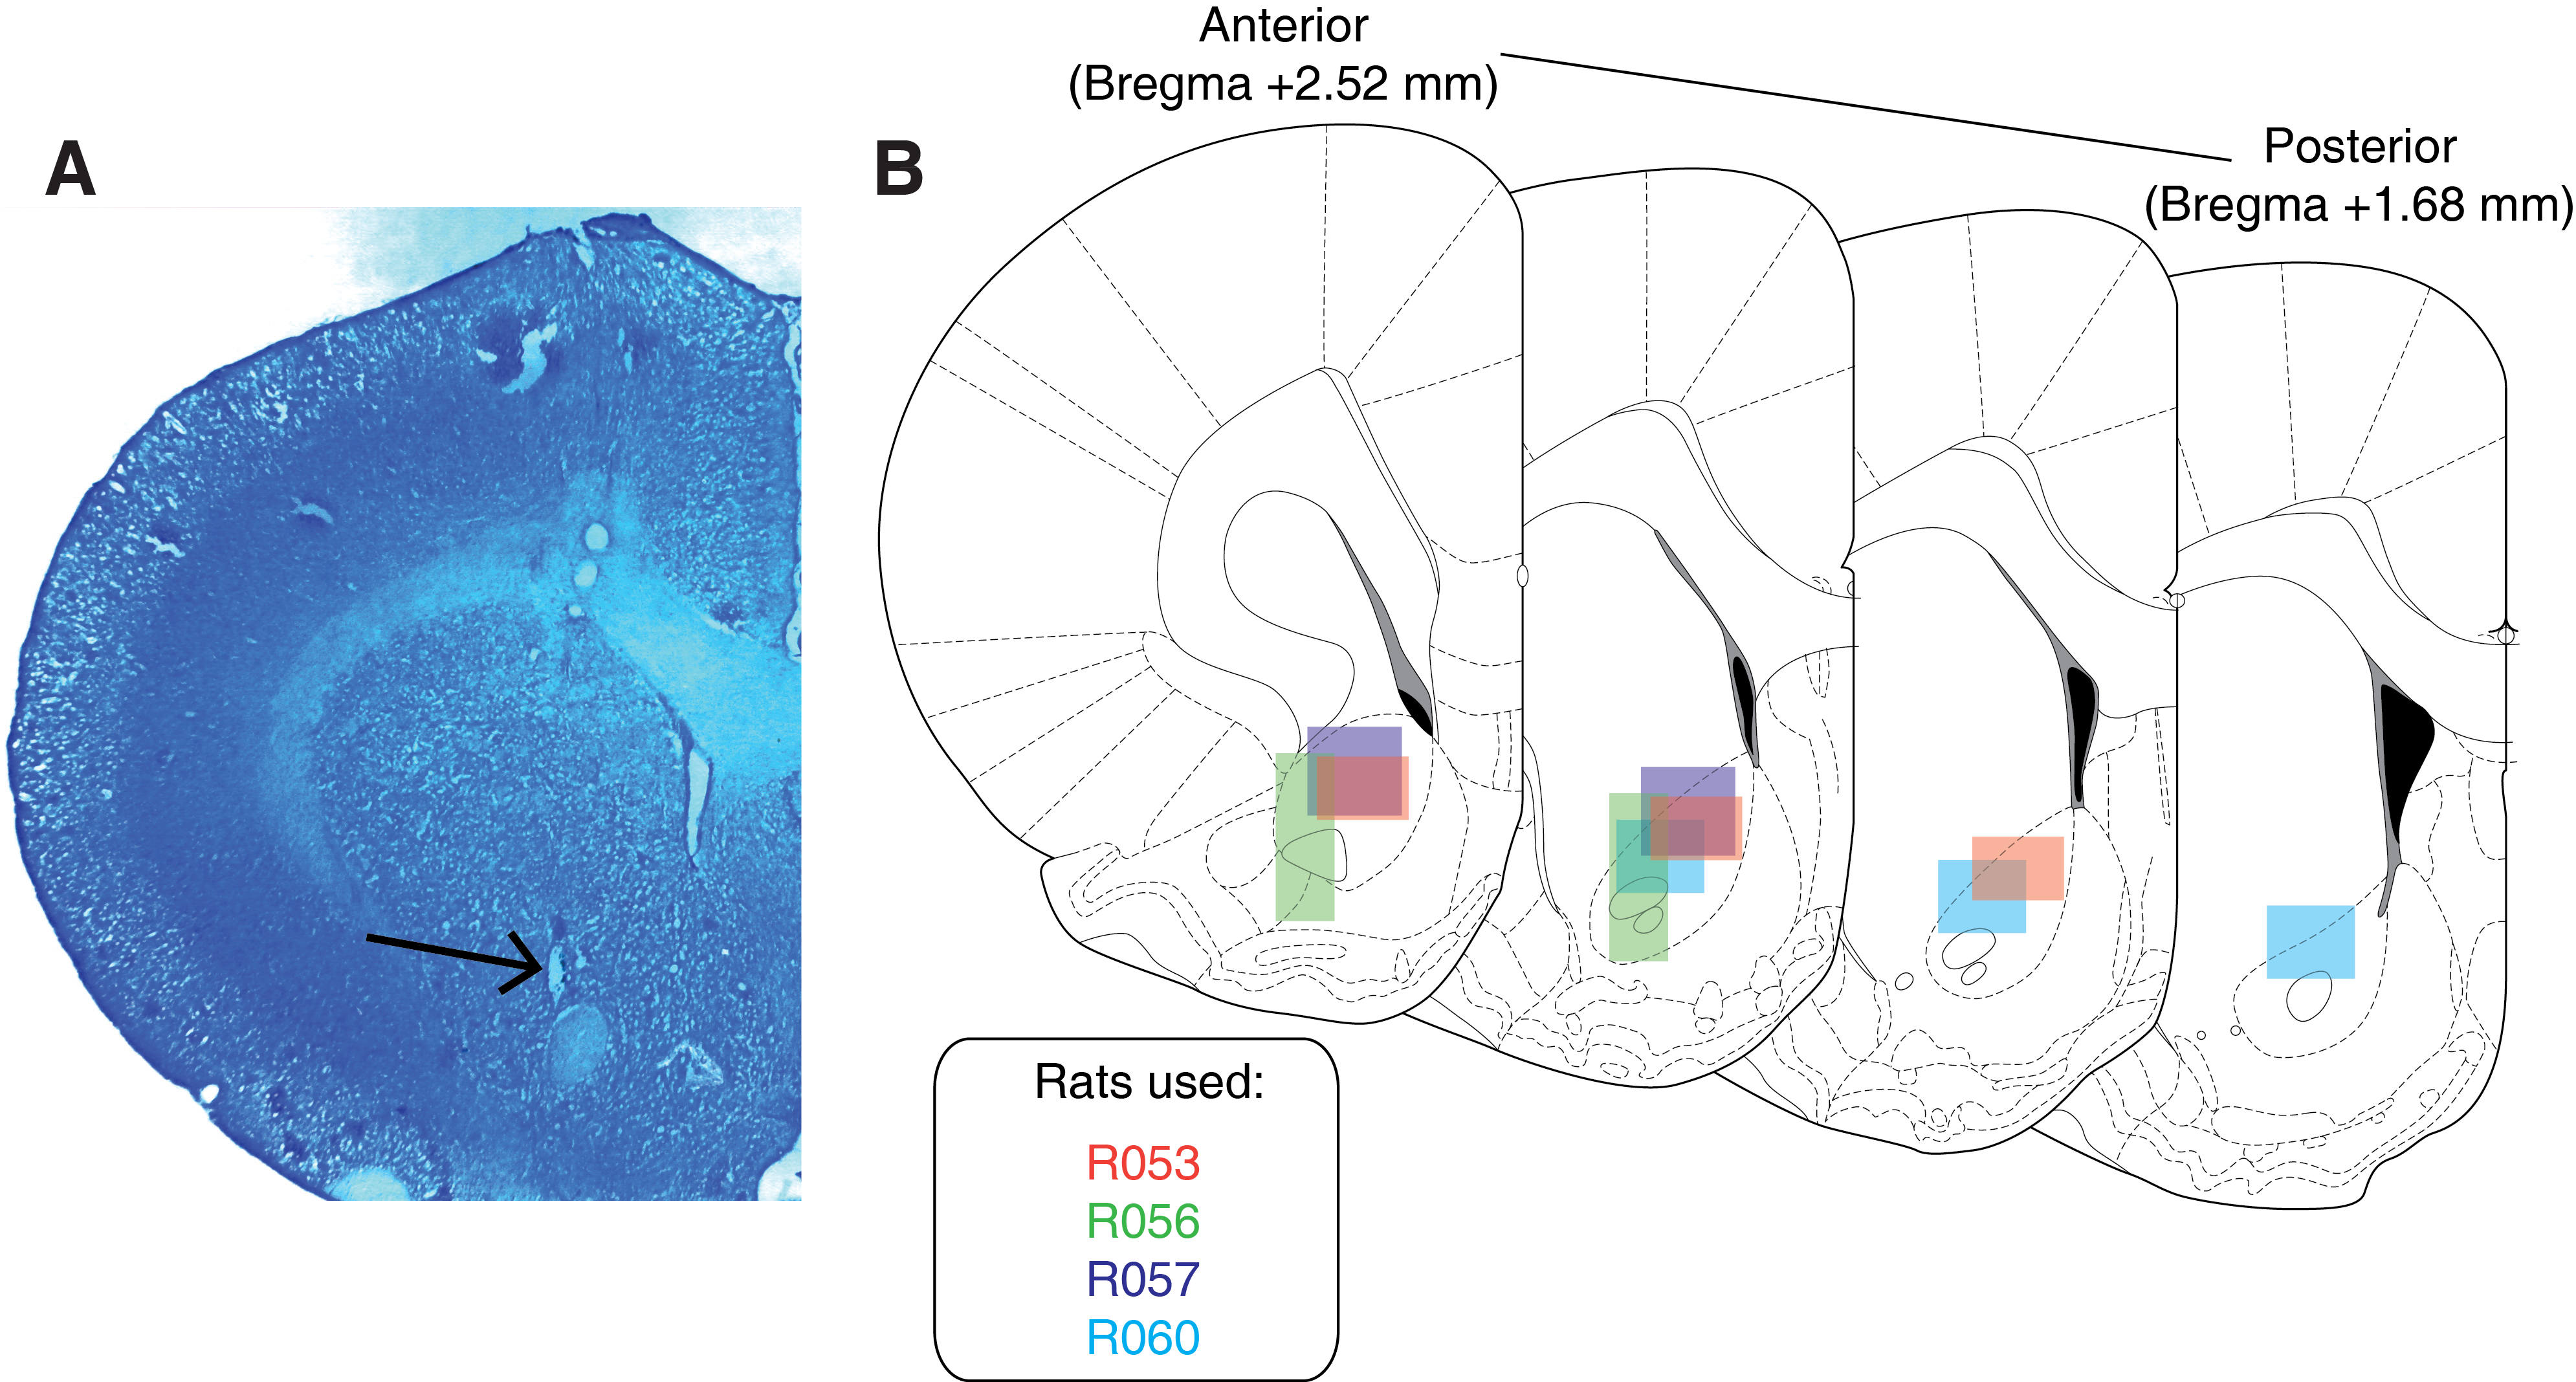
\includegraphics[width=\textwidth]{Fig 3 - Histology.png}
\caption{\DIFdelbeginFL \DIFdelFL{Histology}\DIFdelendFL \DIFaddbeginFL \DIFaddFL{Histological verification of recording sites. Upon completion of experiments, brains were sliced and tetrode placement was confirmed. A. Example section from R060 showing a recording site in the NAc core. B. Schematic showing recording areas for the four rats used in the present study.}\DIFaddendFL }
\label{fig:histo}

\end{figure}
\section*{Results}
% Version 1.2 - Imported from Google Drive
%DIF <  To do JG: add more detail to text, finalize figures after Matt's approval

\subsection*{Behavior}

Rats were trained to discriminate between cues signaling the availability and absence of reward on a square track with four identical arms for two distinct sets of cues. An example learning curve is seen in Figure \ref{fig:behav}A,B. All four rats learned to discriminate between the rewarded and unrewarded cue for both the light and sound blocks as determined by reaching significance (p $<$ .05) on a daily chi-square test comparing approach behavior for rewarded and unrewarded cues for each block, for at least three consecutive days. Linear mixed effects models revealed that cue type had an influence on the likelihood of a rat to make an approach (p $<$ .001), but not for the length of time taken to complete a trial (p $=$ .13)(Figure \ref{fig:behav}C,D).

\begin{figure}[h]
\centering
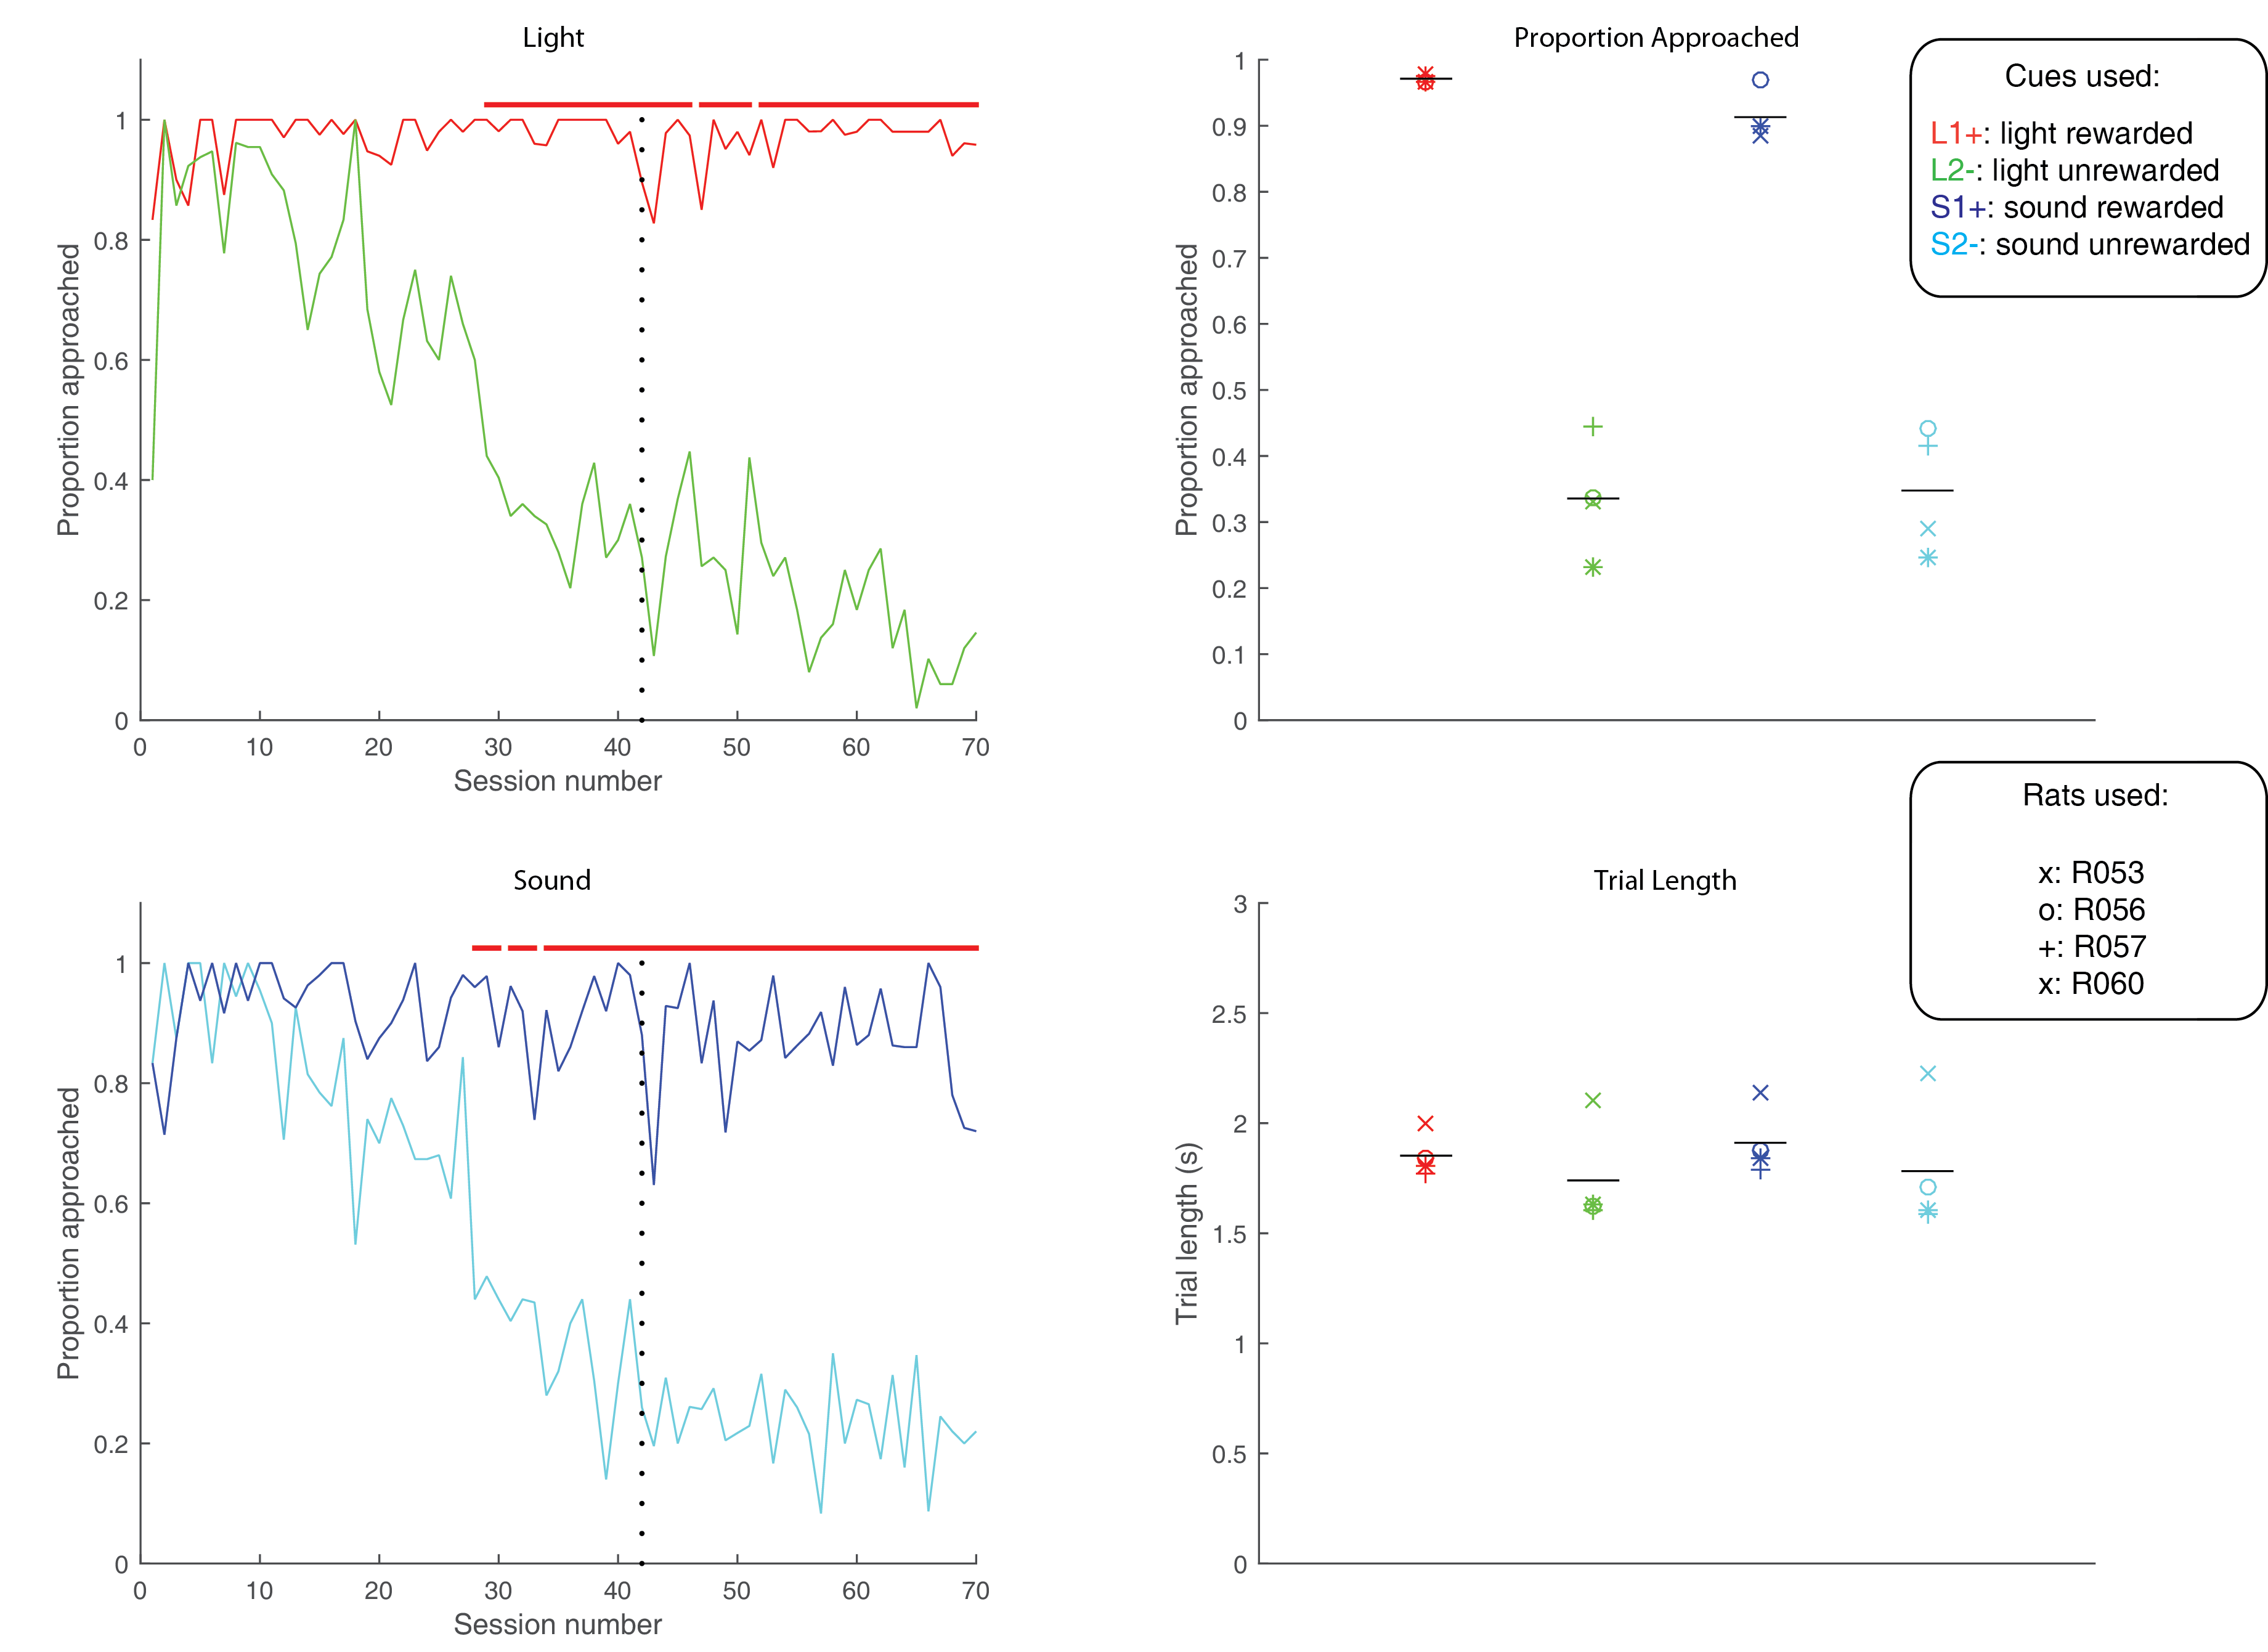
\includegraphics[width=\textwidth]{Fig 4 - Behavioral results.png}
\caption{\DIFdelbeginFL \DIFdelFL{Behavioral results}\DIFdelendFL \DIFaddbeginFL \DIFaddFL{Performance on the behavioral task. A-B. Example learning curves from R060 showing acquisition and maintenance of performance in the light (A) and sound (B) blocks. Dependent measure is proportion of trials approached within a session for a given cue, with a value of 1 being perfect performance for rewarded cues, and 0 being perfect performance for unrewarded cues. Red bars indicate days in which a rat statistically discriminated between rewarded and unrewarded cues, determined by a chi square test. Dashed line indicates time of implantation. C-D. Summary of performance during recording sessions for each rat. C. All rats learned to discriminate between the rewarded and unrewarded cues within a block as measured by a comparison of linear mixed effects models, interpreted as a decreased likelihood to make an approach for an unrewarded cue. D. Average length of time to complete a trial for each cue. Rats on average showed a comparable length of time to complete a trial regardless of cue.}\DIFaddendFL }
\label{fig:behav}
\end{figure}
\subsection*{NAc neurons encode behaviorally relevant and irrelevant cue features}

{\bf General responses to cue:}

A total of 443 units were recorded in the NAc from 4 rats over 57 sessions (Table \ref{tbl1}). The activity of 133 (30\%) of these was modulated by the cue, with more units showing a decrease in firing (n = 124) than an increase (n = 47) around the time of cue-onset (Table \ref{tbl2}). Within this group, 32 were classified as HFNs, while 139 were classified as SPNs. Fitting a GLM to each unit revealed that a variety of task parameters accounted for a significant portion of firing rate variance in NAc cue-modulated units (\DIFdelbegin \DIFdel{Figure \ref{fig:GLM}, \ref{fig:RSQ}}\DIFdelend \DIFaddbegin \DIFadd{Figures \ref{fig:exmaples}, \ref{fig:GLM}}\DIFaddend ). Notably, there were units that discriminated between whether the rat was performing in the light or sound block, which arm the rat was currently on, and whether the rat was engaged in a rewarded or unrewarded trial (Figure \ref{fig:examples}A-F). Interactions between multiple cue features appeared as significant predictors of firing rate variance for 9\% cue-modulated units, although this effect was relatively modest (Figure \ref{fig:examples}G,H). Fitting a GLM to all recorded units...*Jimmie finish this* (data not shown).


\begin{table}
[p]
\centering
\setlength{\tabcolsep}{1 em} % for the horizontal padding
\begin{tabular}{l c  c c c c}

Rat                                  & Total        & MSN (increasing)        & MSN (decreasing)        &FSI (increasing)        &FSI (decreasing)\\
\hline
R053                       & 145         & 51          & 79          & 4         & 11\\
\hline
R056                       & 70         & 12          & 13         & 17          & 28\\
\hline
R057   	          & 136         & 55          & 75          & 3          & 3\\
\hline
R060                       & 92         & 37          & 49          & 3          & 3\\
\hline   

\end{tabular}
\caption {Cells from each rat} \label{tbl1} 
\end{table}

\begin{table}
[p]
\centering
\setlength{\tabcolsep}{1 em} % for the horizontal padding
\begin{tabular}{l c  c c c c}

Task parameter                                 & Total        & MSN (increasing)        & MSN (decreasing)        &FSI (increasing)        &FSI (decreasing)\\
\hline
All cells                       & 443        & 155         & 216          & 27          & 45\\
\hline
Cue modulated                       & 133         &24          &85          & 6          &18\\
\hline
Cue modality       & 37         & 7          & 21          & 1          & 8\\
\hline
Cue location       & 50         &13          & 27          & 3          & 7\\
\hline
Cue outcome       & 34         & 10          & 18        & 0          & 6\\
\hline
Approach behavior      & 31         & 8          & 18          & 1          & 4\\
\hline
Trial length       & 25        & 5          & 18         & 0         & 2\\
\hline
Trial number       & 32         & 11          & 12         & 1          & 8\\
\hline
Recent trial history       & 5         & 0          &5          & 0          & 0\\
\hline
Cue x cue interactions       & 11         & 3          & 7          & 0          & 1\\
\hline
Cue x behavior interactions       & ?         & ?          & ?          & ?          & ?\\
\hline

\end{tabular}
\caption {Cells from GLM} \label{tbl2} 
\end{table}
\begin{figure}[h]
\centering
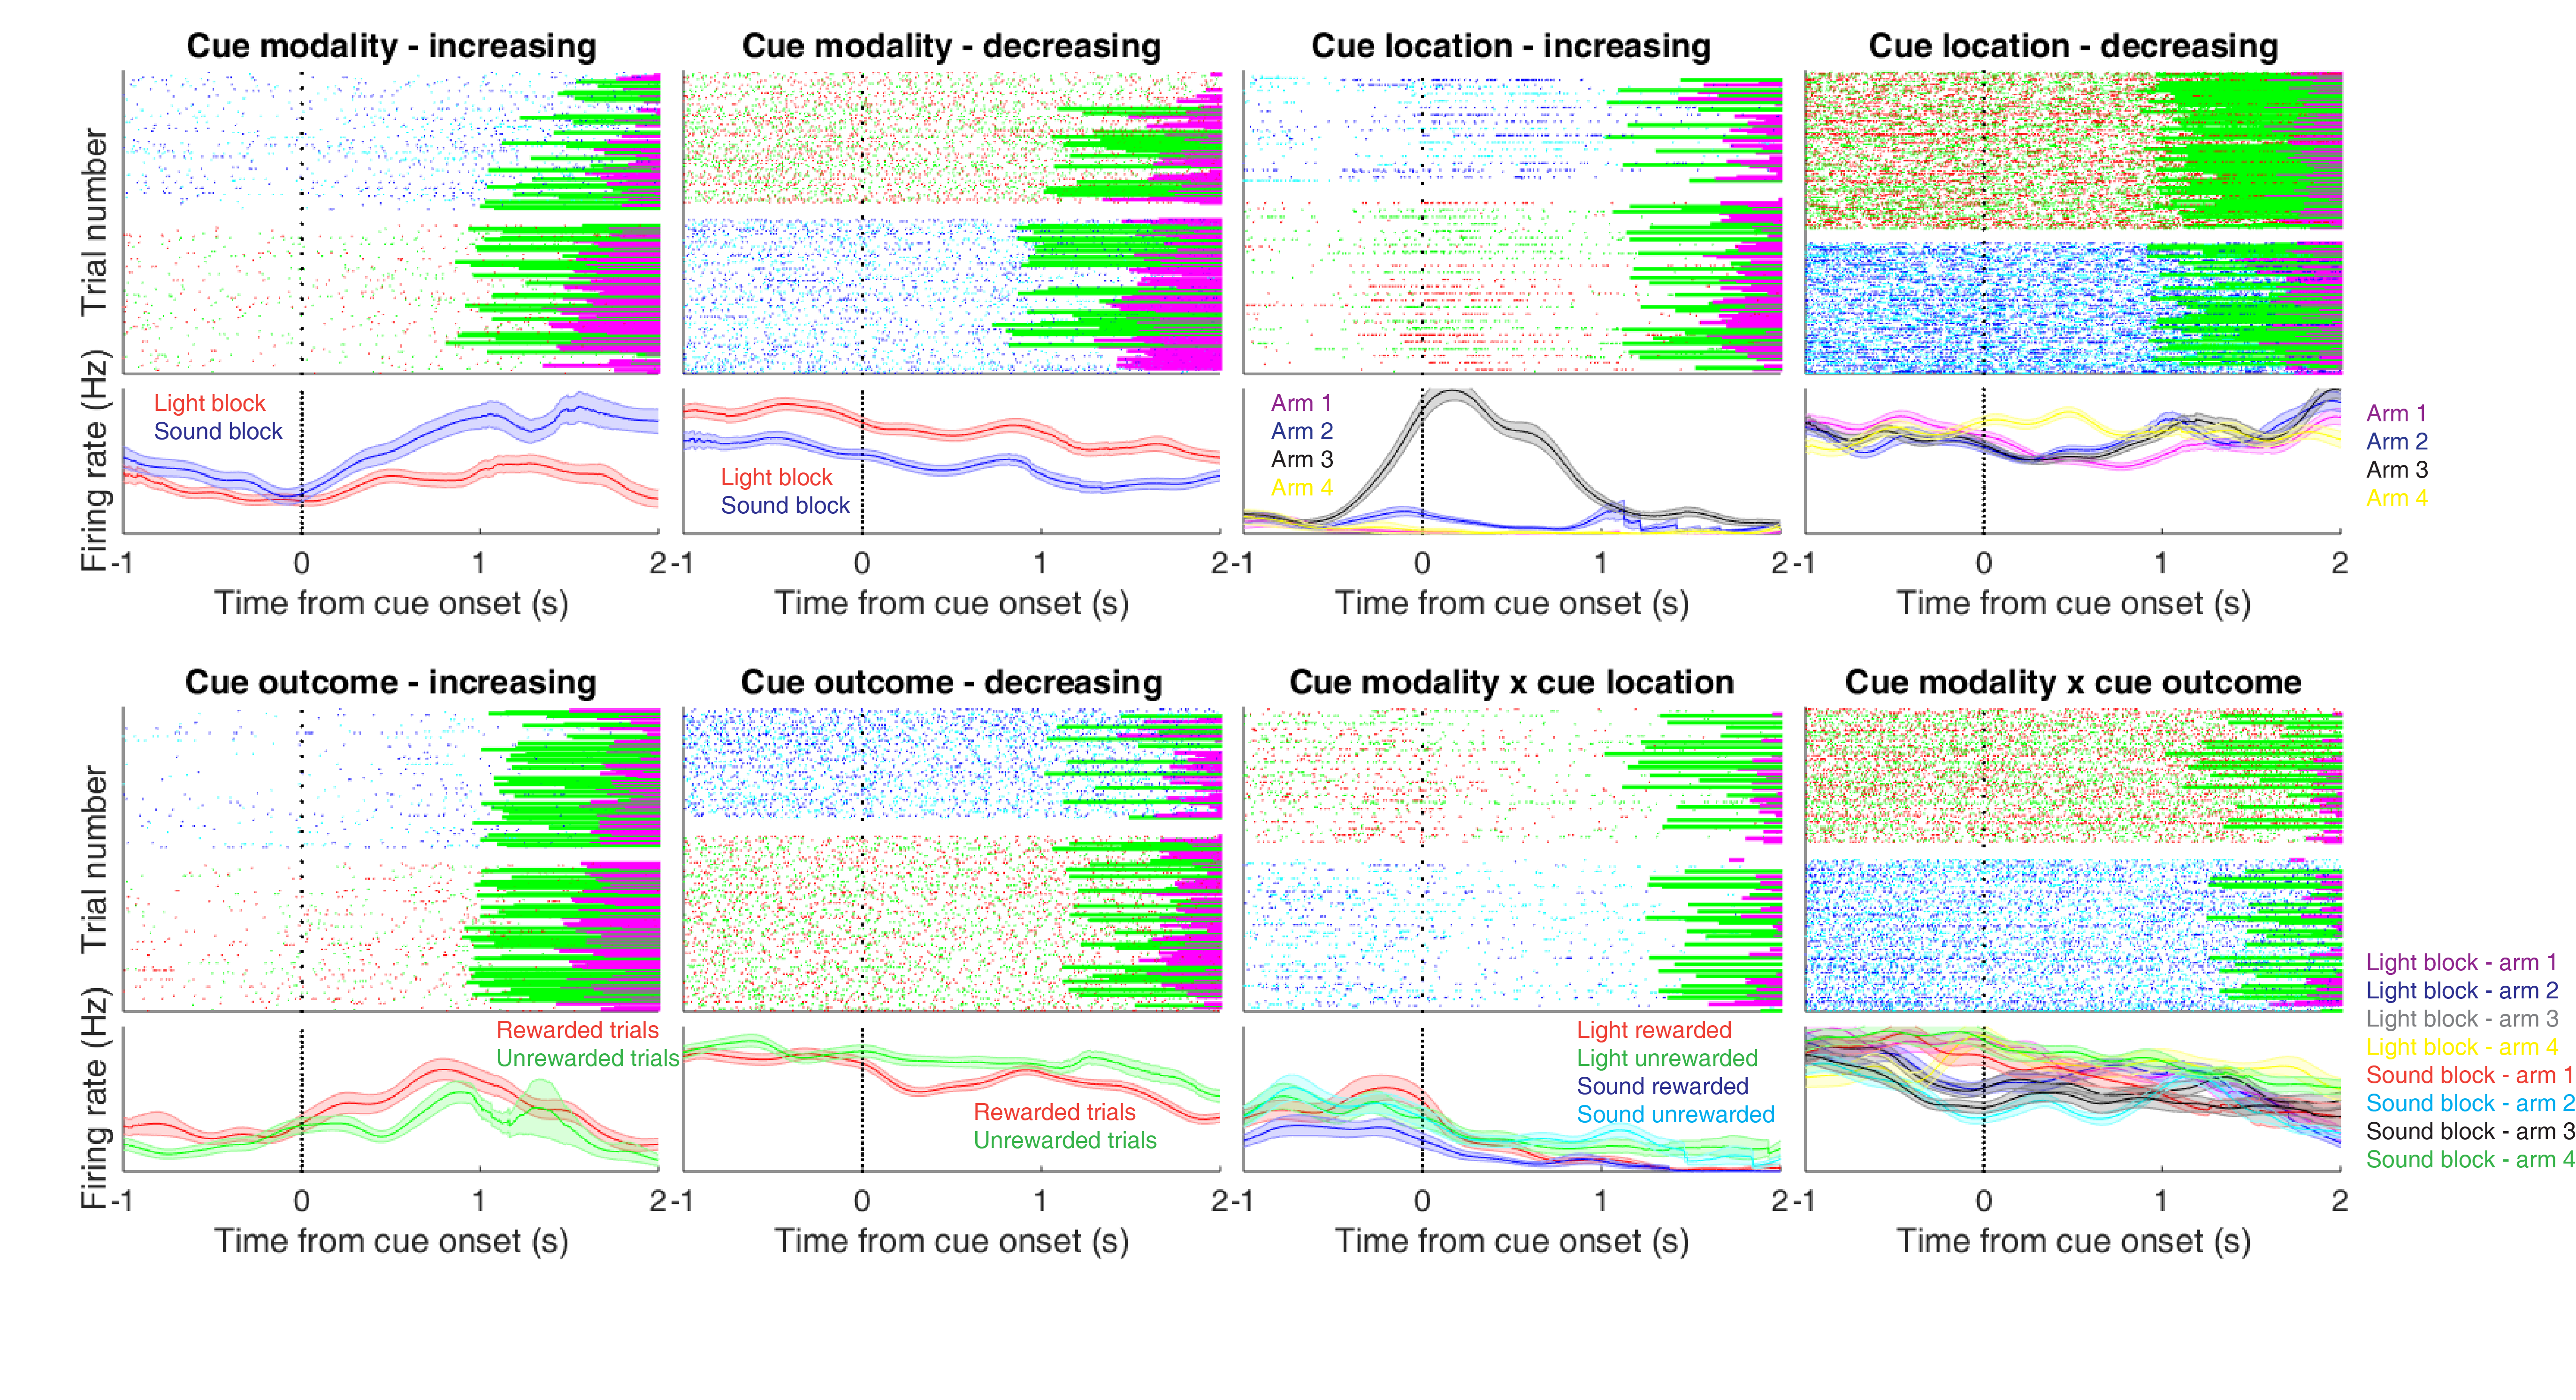
\includegraphics[width=\textwidth]{Fig 5 - Neural examples.png}
\caption{\DIFdelbeginFL \DIFdelFL{Neural }\DIFdelendFL \DIFaddbeginFL \DIFaddFL{Individual }\DIFaddendFL examples \DIFaddbeginFL \DIFaddFL{of NAc units influenced by various task parameters. A. Example of a NAc unit that showed an increase in firing in response to the cue, and whose activity was influenced by which block the rat was in. Top: rasterplot showing the spiking activity across all trials aligned to cue-onset. Spikes across trials are color coded according to cue type, using the same scheme as in previous figures. Green and magenta bars indicate trial termination when a rat initiated the next trial or made a nosepoke, respectively. Bottom: PETHs showing the average smoothed firing rate for the unit for light (red) and sound (blue) blocks, aligned to cue-onset. B. Same as A for a unit that showed a decrease in firing. C-D. Same as A-B for cue location, each color in the PETHs represents average firing response for a different cue location. E-F. Same as A-B for cue outcome, with the PETHs comparing rewarded (red) and unrewarded (green) trials. G-H. Example of units who were modulated by both cue modality and location (G) and cue modality and outcome (H) using similar color schemes as the other examples.}\DIFaddendFL }
\label{fig:examples}
\end{figure}

\begin{figure}
[h]
\centering
\DIFdelbeginFL %DIFDELCMD < 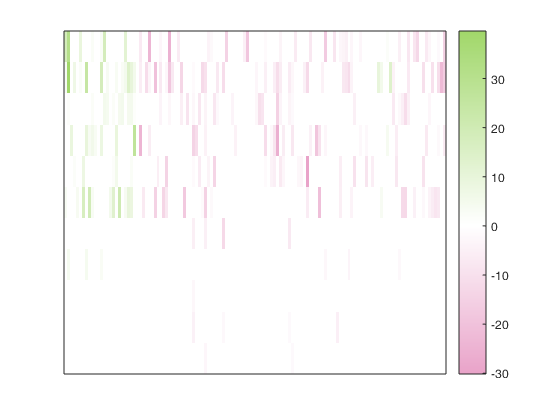
\includegraphics[width=\textwidth]{Fig 6 - GLM matrix.png}
%DIFDELCMD < %%%
\DIFdelendFL \DIFaddbeginFL 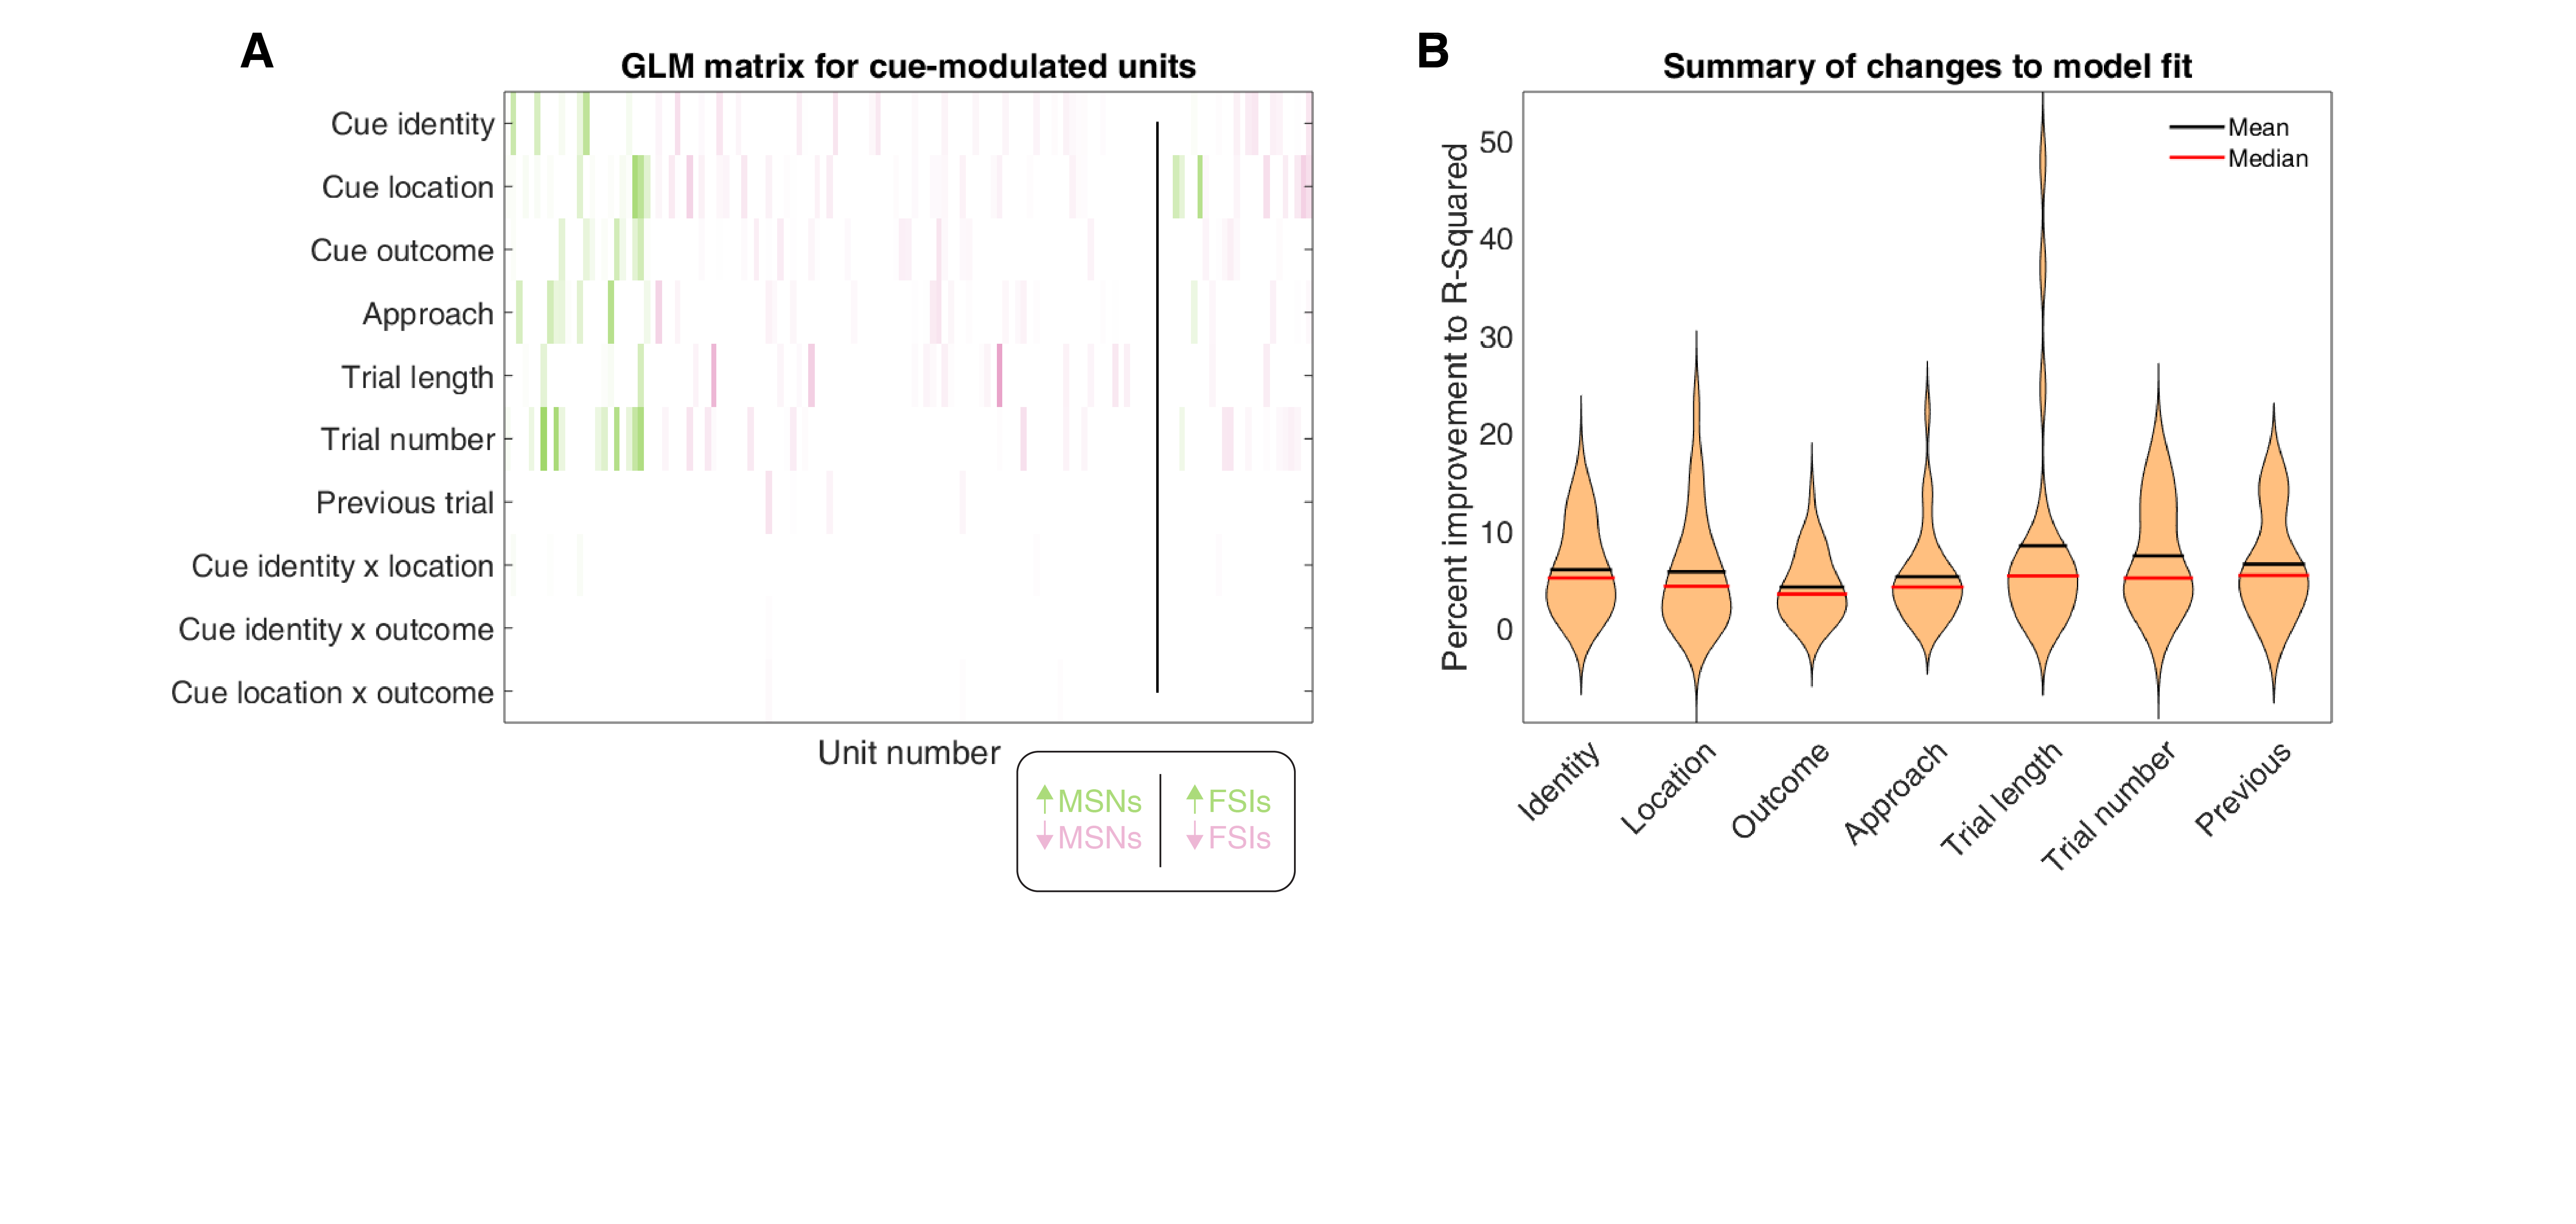
\includegraphics[width=\textwidth]{Fig 6 - GLM.png}
\DIFaddendFL \caption{\DIFaddbeginFL \DIFaddFL{Summary of influence of various task parameters of cue-modulated NAc units after cue-onset. A. }\DIFaddendFL GLM matrix \DIFaddbeginFL \DIFaddFL{demonstrating impact of various task parameters on NAc firing rates. A GLM was fit to each unit that showed evidence of cue modulation by a Wilcoxon signed-rank test. Each row represents a given task parameter, and the x axis shows the influence of the task parameters for each unit, organized from left to right for MSNs that increased firing in response to the cue (green left), MSNs with a decreasing response (red left), FSIs with an increasing response (green right), FSIs with a decreasing response (red right). Response variable is how much of the firing rate variance an individual predictor contributed to the model, as measured by differences in R-squared between the final model and the model minus the predictor of interest. B. Bar graph demonstrating average change in R-squared value with the addition of each of the individual predictors.}\DIFaddendFL }
\label{fig:GLM}

\end{figure}
\DIFdelbegin %DIFDELCMD < \begin{figure}[h]
%DIFDELCMD < \centering
%DIFDELCMD < 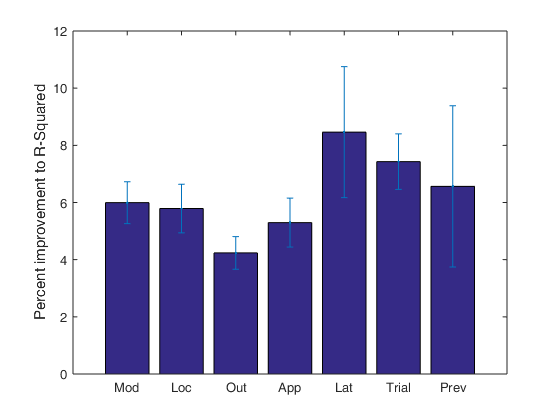
\includegraphics[width=\textwidth]{Fig 6b - RSquared.png}
%DIFDELCMD < %%%
%DIFDELCMD < \caption{%
{%DIFAUXCMD
\DIFdelFL{Average improvement to R-Squared for addition of each parameter. Matt: Was thinking of merging this with the prior GLM matrix, is this worth taking up figure space?}}
%DIFAUXCMD
%DIFDELCMD < \label{fig:RSQ}
%DIFDELCMD < \end{figure}
%DIFDELCMD < 

%DIFDELCMD < %%%
\DIFdelend {\bf Population level responses:}

To get a sense of how cue information was encoded at the population level, firing activity for each unit modulated by a cue feature was z-scored, then the population average for a cue feature was aligned to cue-onset was generated (Fig \ref{fig:pop}). This visualization of the data revealed units whose activity was modulated by cue modality showed a difference in firing rate across blocks that extended beyond the transient response to the cue (Figure \ref{fig:pop}A,B). Additionally, units whom had exhibited a decrease in firing in response to the cue and whose activity was modulated by cue outcome, showed a sustained response that extended beyond cue-onset (Figure \ref{fig:pop}F).  

\begin{figure}[h]
\centering
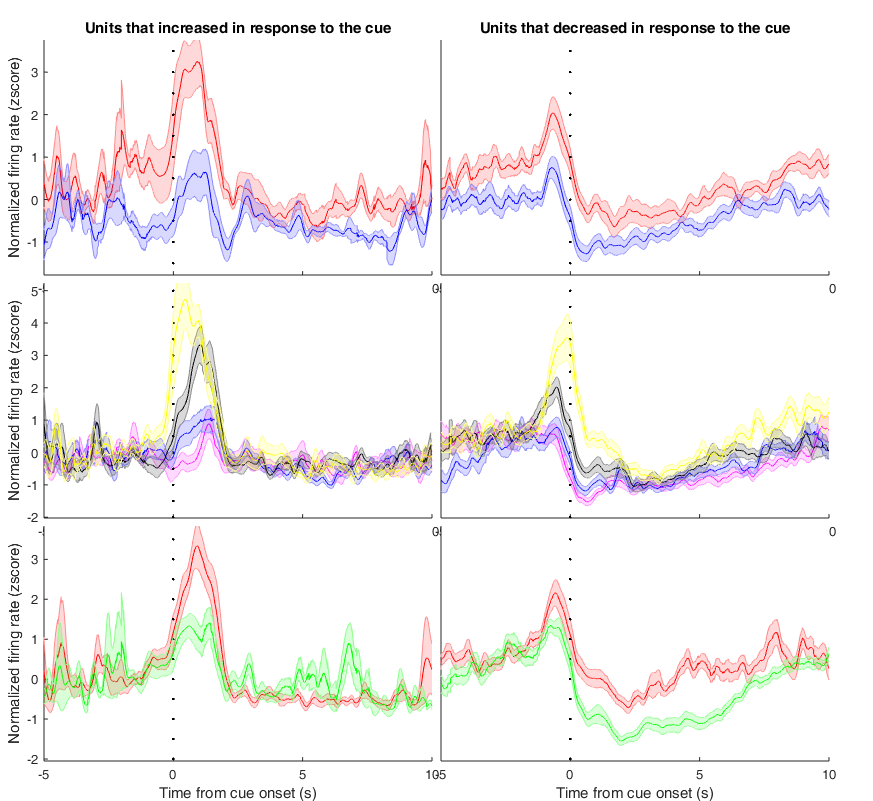
\includegraphics[width=\textwidth]{Fig 7 - Population averages.png}
\caption{\DIFdelbeginFL \DIFdelFL{Population }\DIFdelendFL \DIFaddbeginFL \DIFaddFL{Population-level }\DIFaddendFL averages \DIFaddbeginFL \DIFaddFL{of cue feature sensitive NAc units. A. Average normalized activity for cue-modulated units where cue modality was a significant predictor in the GLM, aligned to cue-onset. Activity is plotted for preferred block (red) and nonpreferred block (blue. B. Same as but for units that decreased in firing. C-D. Same as A-B for cue location. Activity is plotted from most preferred arm (yellow), in decreasing order to least preferred arm (black, navy blue, magneta, respectively). E-F. Same as A-B for cue outcome. Activity is plotted for preferred expected outcome (red), and nonpreferred outcome (green).}\DIFaddendFL }
\label{fig:pop}
\end{figure}
{\bf NAc units segment the task:}

NAc neurons have been shown to have correlates across an entire task space. To look at the distribution of responses throughout our task space and see if this distribution is modulated by cue features, we z-scored the firing rate of each unit and plotted the normalized firing rates of all units aligned to cue-onset and according to peak firing rate. We did this separately for both the light and sound blocks, and found a nearly uniform distribution of firing fields in task space that was not limited to alignment to the cue (Figure \ref{fig:tiling}). Furthermore, to see if this population level activity was similar across blocks, we also organized firing during the sound blocks according to the ordering derived from the light blocks. This revealed, that the overall firing was qualitatively different across the two blocks. Additionally, given that the majority of our units showed an inhibitory response to the cue, we also plotted the firing rates according to the lowest time in firing. This process was repeated for cue location and cue outcomes. 

\begin{figure}[h]
\centering
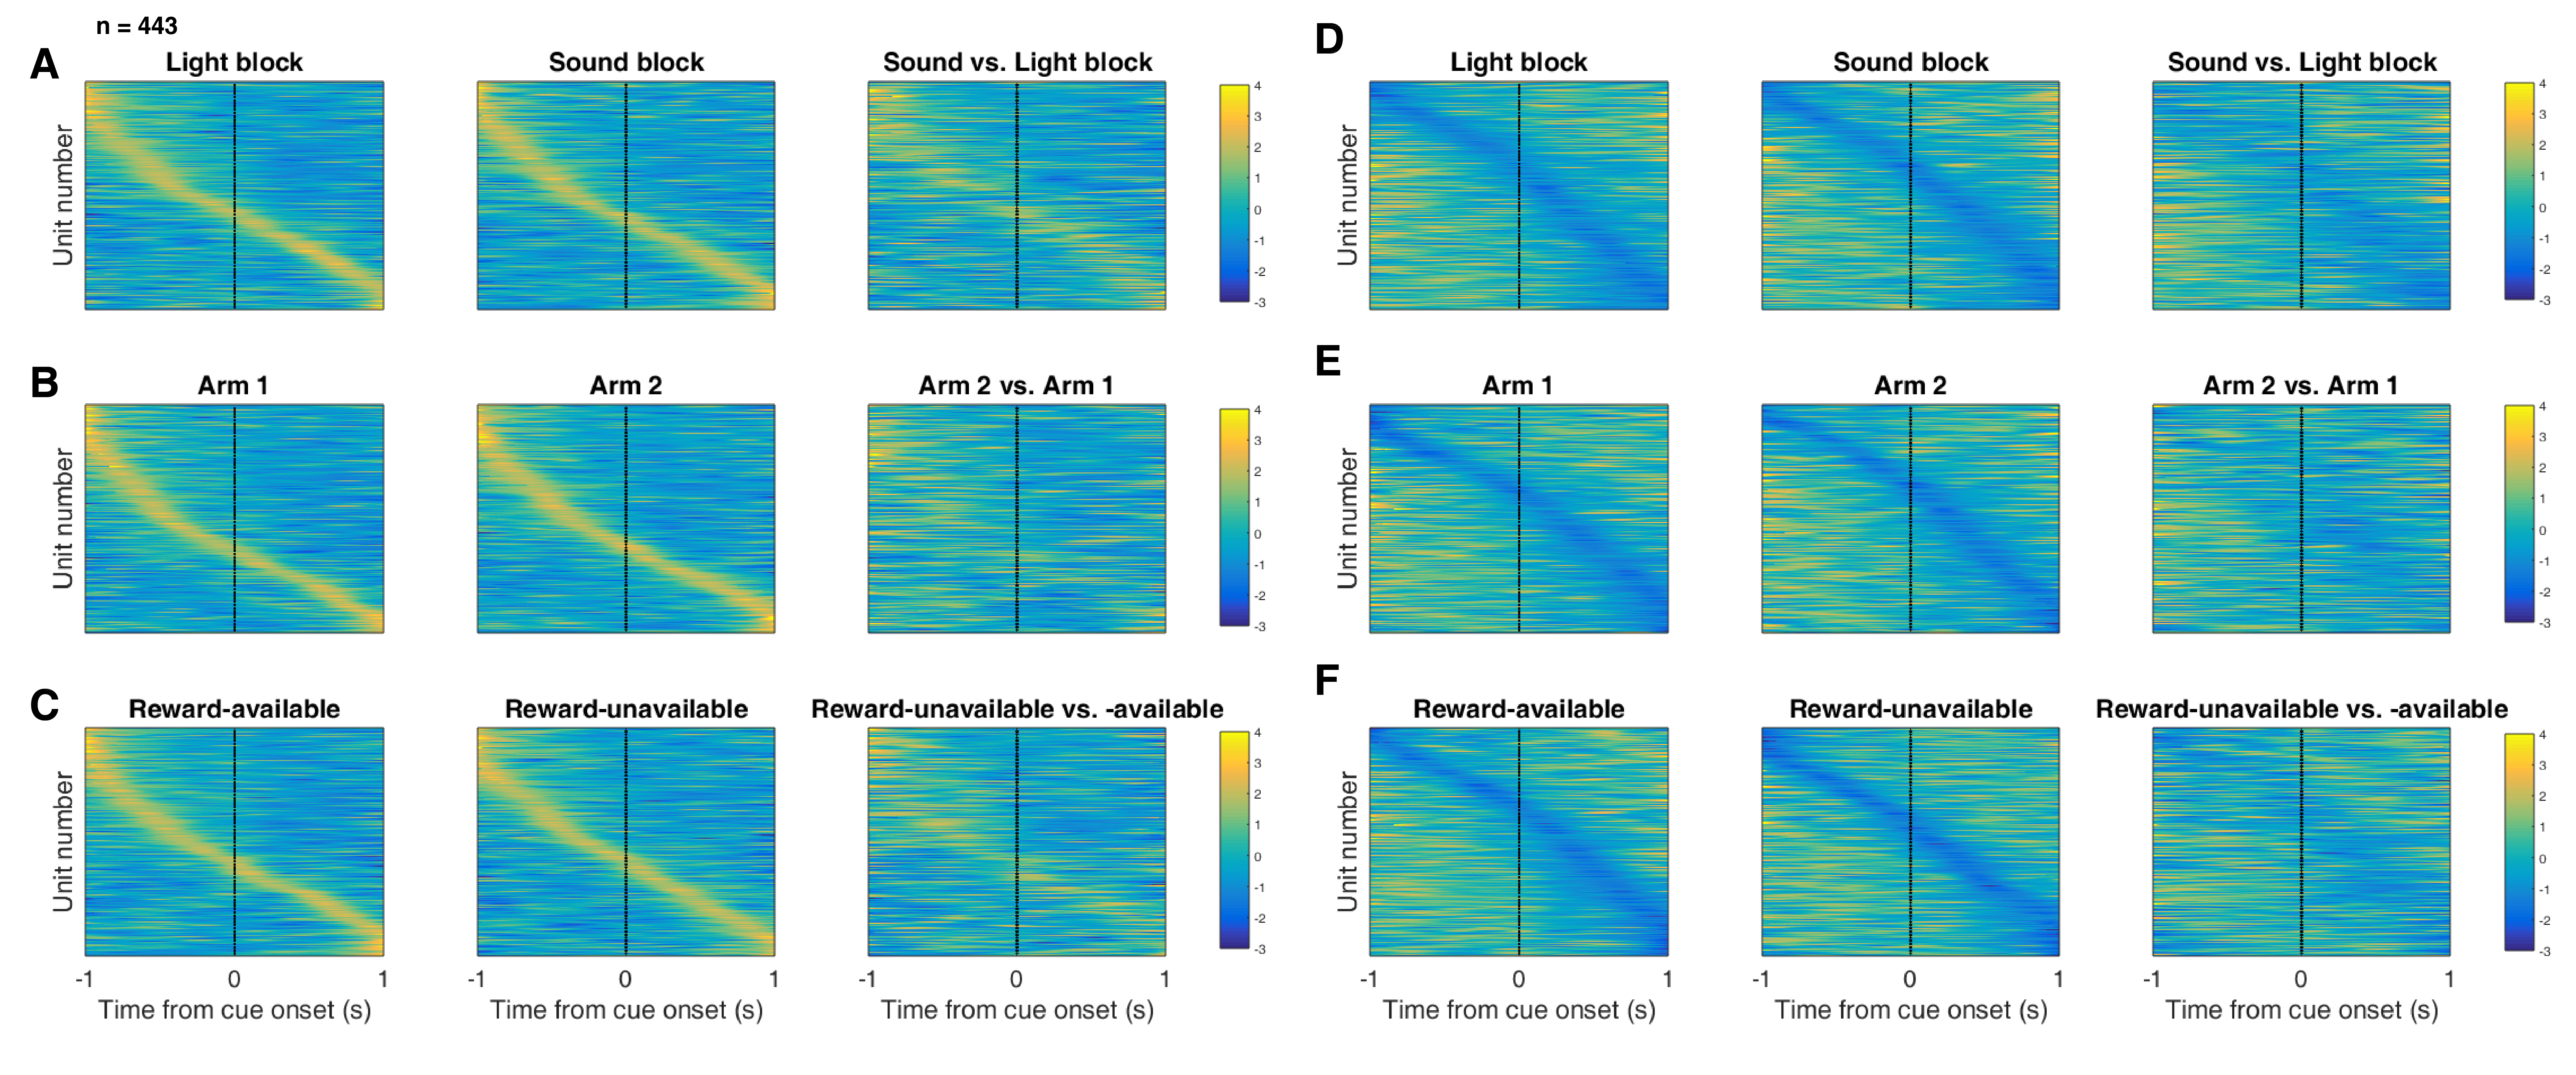
\includegraphics[width=\textwidth]{Fig 8 - Task tiling.png}
\caption{\DIFdelbeginFL \DIFdelFL{Task tiling}\DIFdelendFL \DIFaddbeginFL \DIFaddFL{Distribution of NAc firing rates across task space surrounding cue-onset. A. Firing rates for all recorded units were normalized and ordered according according to peak firing rates for light block (left) and sound block (right), aligned to cue-onset. Middle: Distribution of sound block firing rates using ordering for light block. B. Same as A but ordered according to minimum firing rate. C-D. Same as A-B for a comparison of two cue locations. E-F Same as A-B for comparison of rewarded and unrewarded cues.}\DIFaddendFL }
\label{fig:tiling}
\end{figure}
{\bf Encoding of cue features is not limited to cue-onset:}

In order to be useful for learning, a trace of the cue must be maintained until the outcome. Fitting a GLM to the firing rates of cue-modulated units at the time of a nosepoke response showed that a variety of units still discriminated firing according to various cue features, but not other task parameters (Table \ref{tbl3}, Figures \ref{fig:NP_GLM}, \DIFdelbegin \DIFdel{\ref{fig:NP_RSQ}, }\DIFdelend \ref{fig:NP_pop}). Fitting a GLM to all recorded units...*Jimmie finish this* (data not shown). Furthermore, aligning normalized peak firing rates to nosepoke onset, revealed a clustering of responses around reward receipt (Figure \ref{fig:NP_tiling}). Alongside this, fitting a GLM to the firing rates of cue-modulated units at the time of reward receipt, revealed 10 units (8\%) where cue outcome accounted for an average of 32\% of firing rate variance (data not shown). 


\begin{table}
[p]
\centering
\setlength{\tabcolsep}{1 em} % for the horizontal padding
\begin{tabular}{l c  c c c c}

Task parameter                                 & Total        & MSN (increasing)        & MSN (decreasing)        &FSI (increasing)        &FSI (decreasing)\\
\hline
Cue modality       & 66         &14          & 36          & 2          &14\\
\hline
Cue location       & 66         &14          & 40          & 3          & 9\\
\hline
Cue outcome       & 42        & 8          & 29        & 0          & 5\\
\hline
Trial length       & 0        & 0         & 0         & 0         & 0\\
\hline
Trial number       & 0         & 0          & 0         & 0          & 0\\
\hline
Recent trial history       & 0         & 0          &0          & 0          & 0\\
\hline
Cue x cue interactions       & 0         &0          & 0          & 0          & 0\\
\hline
Cue x behavior interactions       & 0         & 0          & 0          & 0          & 0\\
\hline

\end{tabular}
\caption {Cells from nosepoke GLM} \label{tbl3} 
\end{table}

\begin{figure}
[h]
\centering
\DIFdelbeginFL %DIFDELCMD < 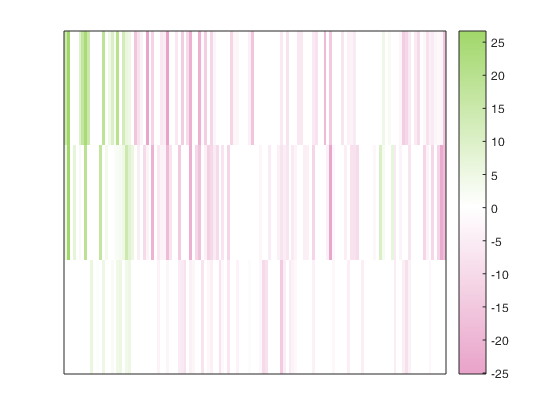
\includegraphics[width=\textwidth]{Fig 9 - NP GLM matrix.png}
%DIFDELCMD < %%%
\DIFdelendFL \DIFaddbeginFL 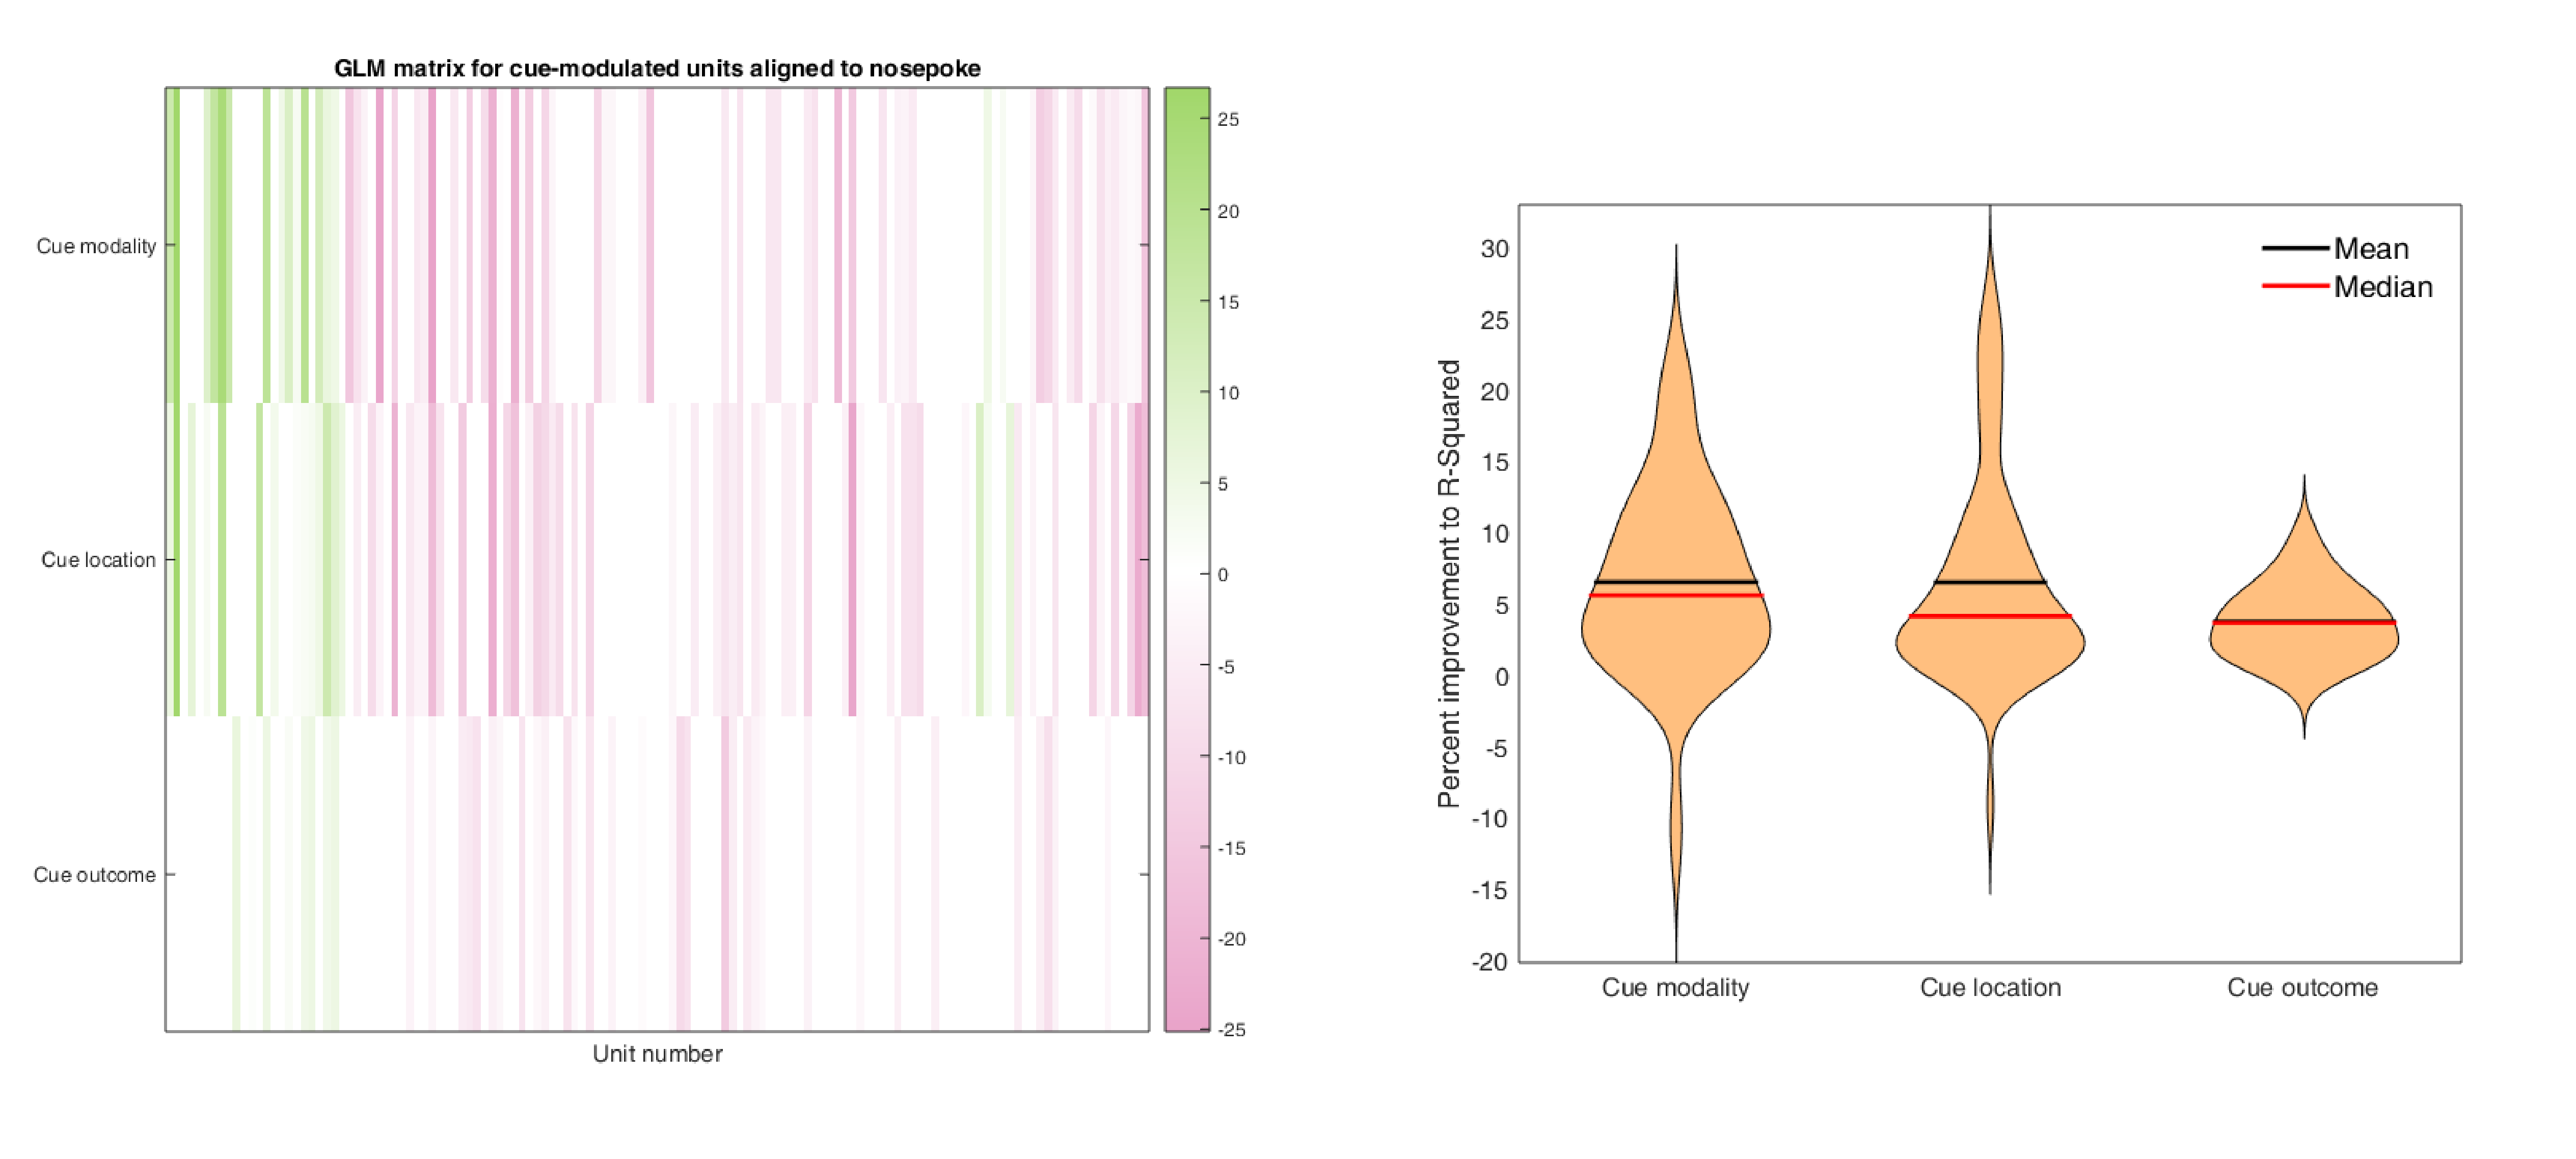
\includegraphics[width=\textwidth]{Fig 9 - NP GLM.png}
\DIFaddendFL \caption{\DIFdelbeginFL \DIFdelFL{NP }\DIFdelendFL \DIFaddbeginFL \DIFaddFL{Summary of influence of various task parameters of cue-modulated NAc units during nosepoke. A. }\DIFaddendFL GLM matrix \DIFaddbeginFL \DIFaddFL{demonstrating impact of various task parameters on NAc firing rates. A GLM was fit to each unit that showed evidence of cue modulation by a Wilcoxon signed-rank test. Each row represents a given task parameter, and the x axis shows the influence of the task parameters for each unit, organized from left to right for MSNs that increased firing in response to the cue (green left), MSNs with a decreasing response (red left), FSIs with an increasing response (green right), FSIs with a decreasing response (red right). Response variable is how much of the firing rate variance an individual predictor contributed to the model, as measured by differences in R-squared between the final model and the model minus the predictor of interest. B. Bar graph demonstrating average change in R-squared value with the addition of each of the individual predictors.}\DIFaddendFL }
\label{fig:NP_GLM}
\end{figure}

\begin{figure}
[h]
\centering
\DIFdelbeginFL %DIFDELCMD < 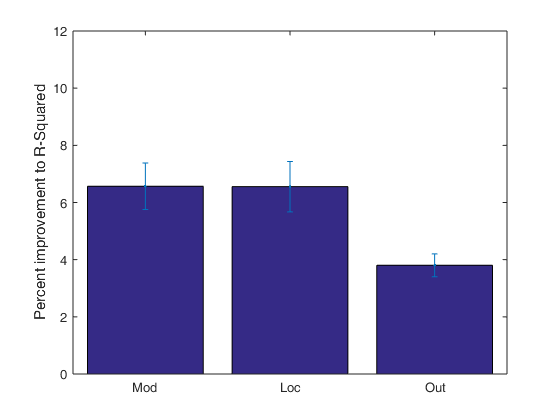
\includegraphics[width=\textwidth]{Fig 9b - RSquared.png}
%DIFDELCMD < %%%
%DIFDELCMD < \caption{%
{%DIFAUXCMD
\DIFdelFL{NP RSquared}}
%DIFAUXCMD
%DIFDELCMD < \label{fig:NP_RSQ}
%DIFDELCMD < \end{figure}
%DIFDELCMD < 

%DIFDELCMD < \begin{figure}[h]
%DIFDELCMD < \centering
%DIFDELCMD < %%%
\DIFdelendFL 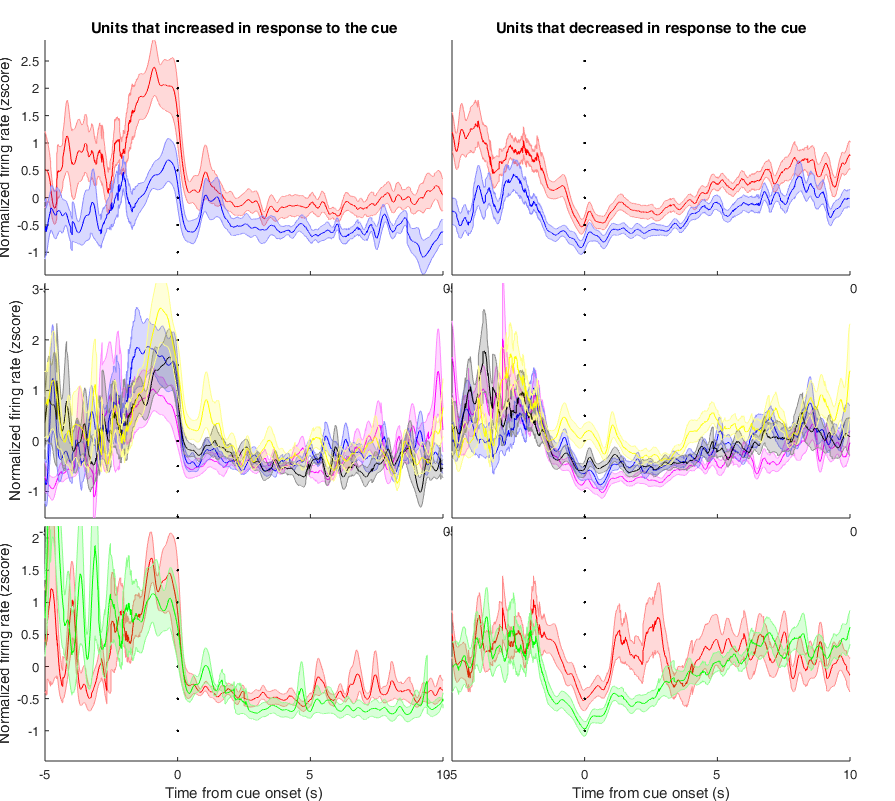
\includegraphics[width=\textwidth]{Fig 10 - NP population averages.png}
\caption{\DIFdelbeginFL \DIFdelFL{NP population }\DIFdelendFL \DIFaddbeginFL \DIFaddFL{Population-level }\DIFaddendFL averages \DIFaddbeginFL \DIFaddFL{of cue feature sensitive NAc units during a nosepoke. A. Average normalized activity for cue-modulated units where cue modality was a significant predictor in the GLM, aligned to nosepoke with reward delivery occurring 1 s after nosepoke. Activity is plotted for preferred block (red) and nonpreferred block (blue. B. Same as but for units that decreased in firing. C-D. Same as A-B for cue location. Activity is plotted from most preferred arm (cyan), in decreasing order to least preferred arm (navy blue, green, red, respectively). E-F. Same as A-B for cue outcome. Activity is plotted for preferred expected outcome (red), and nonpreferred outcome (green).}\DIFaddendFL }
\label{fig:NP_pop}
\end{figure}
\begin{figure}
[h]
\centering
\includegraphics[width=\textwidth]{Fig 11 - NP task tiling.png}
\caption{\DIFdelbeginFL \DIFdelFL{NP }\DIFdelendFL \DIFaddbeginFL \DIFaddFL{Distribution of NAc firing rates across }\DIFaddendFL task \DIFdelbeginFL \DIFdelFL{tiling}\DIFdelendFL \DIFaddbeginFL \DIFaddFL{space during approach trials. A. Firing rates for all recorded units were normalized and ordered according according to peak firing rates for light block (left) and sound block (right), aligned to nosepoke with reward delivery occurring 1 s after nosepoke. Middle: Distribution of sound block firing rates using ordering for light block. B. Same as A but ordered according to minimum firing rate. C-D. Same as A-B for a comparison of two cue locations. E-F Same as A-B for comparison of rewarded and unrewarded cues.}\DIFaddendFL }
\label{fig:NP_tiling}

\end{figure}
\section*{Discussion}
% Version 1.2 - Imported from Google Drive
% To do JG: restructure to fit new results layout, add references

The present study found evidence for coding of multiple identifying features of motivationally relevant stimuli; the sensory modality of the presented cue, as well at its physical location within the track. Furthermore, this coding was both independent, and intermixed with coding for the associated outcome of the cue as well as motivational vigor, measured by time to complete the trial. At the population level, a tiling of task structure was observed such that all points within our analyzed task space was accounted for by the ordered peak firing rates of all cells, and this tiling differed between blocks where sound or light cues were presented.
Cells that discriminated across blocks were not simply due to drifting of the signal across trials, as cells that showed a drift in firing between the first and second half within a block were excluded from the analysis. Furthermore, even though actions were stereotyped during correct trials, such that the rat always turned left at the decision point to approach for reward, and right to skip the receptacle and initiate the next trial, cells that were modulated by the expected value of the cue maintained their specific firing patterns even during error trials where the rat turned left after presentation of the unrewarded cue, suggesting that these signals did not represent action values. Additionally, NAc signals have been shown to be modulated by response vigor, to detangle this from our results we included the trial length as a predictor in our GLMs, and found cells with correlates independent of trial length.

{\bf Cue modality:}  

Our finding that ventral striatal units can discriminate between cues from different sensory modalities expands upon an extensive literature examining neural correlates of conditioned stimuli. Perhaps the most comparable work in rodents comes from a study that found distinct coding for an odor when it predicted separate but equally valued rewards (Cooch). The present work is complementary to this as it shows that ventral striatal cells have representations of identifiable aspects of the cue itself, in addition to the reward it predicts. Another study paired separate cues with appetitive or aversive outcomes, and found separate populations of cells that encode each cue, with many switching selectivity after reversal of the associations between the cues and outcomes, providing evidence that the NAc encodes the biological significance of stimuli. Once again, our study was different as we recorded neural responses to distinct cues encoding the same anticipated outcome, suggesting that even when the biological relevance of these stimuli is similar, the NAc dissociates their representations at the level of the single-unit (Setlow). Another possibility is that these modality specific cells were encoding the context, rule, or sequence within a session as some cells responded similar for both rewarded and unrewarded cues within a block. This interpretation is in alignment with a recent paper from the primate realm that recorded ventral striatal responses during the Wisconsin Card Sorting Task (WCST), a common set-shifting task used in both the laboratory and clinic, and found cells that preferred firing to stimuli when a certain rule, or rule category was currently active (Sleezer). Indeed, an encoding of the current strategy could be an explanation as to why differentially tiling of task structure was observed across blocks in the current study. Further support for a modulation of NAc responses by strategy comes from an fMRI study that examined BOLD levels during a set-shifting task (FitzGerald et al., 2014). In this task, participants learned two sets of stimuli-reward contingencies, a visual set and auditory set. During testing they were presented with both simultaneously, and the stimulus dimension that was relevant was periodically shifted between the two. Here, they found that bilateral NAc activity reflected value representations of whatever the currently relevant stimulus dimension was, and not the irrelevant stimulus. The current finding of separate, but overlapping, populations of cells encoding cue modality and expected value, suggests that the fMRI finding is generated by the combined activity of several different functional cell types. 

A caveat of the current study is that rats were never presented with both sets of cues simultaneously, and thus never had to switch strategies, although extrapolating the data from the primate study, suggests that the activity of the cue modality cells would be modulated by relevance. Keeping along this theme, the current data set is unable to identity precisely what the modality-sensitive neurons were encoding, that is were they tracking representations of stimulus identity, a preferred context, or even a macroscale representation of progress through the session. Furthermore, their relevance for ongoing behavior is also uncertain. NAc core lesions have been shown to impair shifting between different behavioral strategies, and it is possible that selectively silencing the cells that prefer responding for a given modality or rule would impair performance when the animal is required to use that information, or artificial enhancement of those cells would cause them to use the rule when it is the inappropriate strategy.  

{\bf Encoding of position:} 

Our finding that cue-evoked activity was modulated by cue location sides with some of the literature (Lavoie, 1994; Tabuchi, 2000; Strait, 2016). An alternative explanation for a pure spatial representation, is that these are task segmentation correlates, keeping track of where in the task the rat is. A previous non-human primate paper has shown that when reward is contingent upon completion of a series of trials, separate populations of NAc neurons signal the start of a schedule, subsequent trials in the schedule, and the first trial in extended schedules (Shidara et al., 1998). This signalling of position within a sequence has been observed in subsequent studies, and it is possible that the our rats were keeping track of which specific arm they were in as part of a sequence of arms, and not just strictly a spatial representation (Mulder, 2004 and 2005; Khamassi et al., 2008; Berke, 2009). Also, given that our task is pseudo-random, it is possible that the rats learned which cue to anticipate, and the neural activity could reflect this. However, this is unlikely as including a ‘previous trial’ variable in the analysis did not explain a significant amount of firing rate variance in response to the cue for the vast majority of cells..

{\bf Mixed selectivity:} 

Several other papers have reported unit profiles that integrate different task-related variables. These papers report integrated coding between expected value and subsequent motor responses, expected value and identity of a reward, and a combination of spatial-, movement-, and reward-related features (Roesch, Lavoie, Cooch). However, our study is the first to show mixed selectivity among identifying features of a cue and expected outcome or behavior. The presence of mixed selectivity responses confers a larger number of input-output relationships that are available to a given neuron. A possible functional consequence of this attribute of NAc units, is the combination and transformation of various motivationally relevant features into a signal informing downstream decoders such as the ventral pallidum about appropriate behaviors in obtaining motivationally relevant goals and biasing action selection towards these behaviors. 
Mixed selectivity in the NAc could be a consequence of synaptic integration from a variety of anatomically distinct inputs, as seen in experiments examining the convergence of various NAc afferents at the level of synaptic transmission and stimulation-induced firing (Goto and Grace 2008). In one such experiment it was shown that NAc cells that responded to stimulation of either the fornix, amygdala, or PFC, typically responded to stimulation from all inputs (O’Donnell and Grace, 1995). Furthermore, an interaction between these inputs was observed such that PFC stimulation failed to elicit spiking in the NAc neurons unless they were in a depolarized UP-state, a state induced by hippocampal stimulation and was dependent on an intact fornix. Hippocampal-induced suppression of other inputs has also been observed for the BLA (Mulder et al., 1998). Recently, it has also been shown that train stimulation of PFC afferents reduces hippocampal-evoked NAc responses, suggesting that there is competition between various inputs (Calhoon and O’Donnell, 2013). These studies suggest that the integration of the variables we saw could be the result of this gating observed in behaviorally-independent preparations. However, given that we did not systematically manipulate these various limbic and cortical afferents, comments on the anatomical origins of the observed mixed selectivity responses are speculative at this point.

Integrating cue identity and value, as seen in the present study, could be one neural instantiation of how value is associated with the appropriate predictive stimuli (credit assignment), keeping in mind that value encoding is distributed, redundantly in some aspects, across various structures (Hayden Nat Neuro opinion). Indeed, lesions of the NAc impair the ability to learn changes in reward value or identity in an unblocking experiment, as well as disrupting dopamine RPEs generated by modification of timing of reward (McDannald 2011, Takahashi 2016). Would be interesting to see if uncoupling the integrated coding of stimulus features and predictive properties of a cue has an effect on the ability of a rat to use reward-predictive cues to pursue the associated reward.

{\bf Tiling of task structure:}

 Additionally, we found that the population of recorded units had a relatively uniform distribution of firing fields within our task space, similar to what has been reported previously (Shidara, 1998; Berke, 2009; Lansink, 2012). Uniquely, we found that this representation differed according to whether the rat was currently engaged in the light or sound block, suggesting that this could be a possible neural correlate for encoding the currently relevant strategy in the NAc. During progress through a predictable trial series, neurons represented state value of cue (Shidara 1998). Single-unit responses allowed the monkey to know how it was progressing throughout the task. Likewise, the tiling we saw could be a consequence of upstream cortical or limbic inputs informing the striatum of the current task rules. Another possibility is that the NAc not only pays attention to progress throughout a task within a trial, but also higher-order task information, like blocks. Cue location was a behaviorally irrelevant variable in the current experiment, but it is possible that if this tiling is dependent on hippocampal input, or related to a state value representation, that making cue location a relevant variable by adding positional contingencies such as only alternating arms are rewarded in one block, would result in a further separation of the mapping within a block between the rewarded and unrewarded arms. Furthermore, dopamine levels in the NAc fluctuate through a trial, and it is possible that the observed tiling could be a NAc-representation of state value related to this temporally evolving dopamine signal. Future experiments should monitor this mapping of task structure during the application of dopamine antagonists. Finally, the presence of functional correlates not evident when looking at single-unit responses time-locked to salient task events emphasizes the need to employ ensemble level analyses across all aspects of a task.

%\bibliography{vStrCueCoding}
\end{document}
